
% PAGES: 10
\chapter{Experimental Results and Analysis}
\label{mt:c:expResults}

The following chapters present the examined results and analysed aspects. First the image processing characteristics are analysed with test scenarios, which focus the interesting aspects of investigation. Each test scenario contains beside the description of the investigated domains, also the expected results of the experiments.
These expectations are compared, with the results of the experiments and discussed. After the analysis of the image processing, the chapter 
\ref{mt:c:expResults:AnalysisofControlbehaviour} shows the characteristics and optimisation of the control architecture and the analysis and tune strategy of the control system. Finally the analysis of the position correction scheme in chapter 
\ref{mt:c:expResults:AnalysisofPositionCorrectionScheme}, focus the complete position correction system and combines the previous analysed results together. Thereby different scenarios are executed with different configurations and disturbances. Furthermore a final analysis also demonstrate the hovering state characteristics of the focused configurations.

\section{Analysis of Image Processing}
\label{mt:c:expResults:AnalysisofImageProcessing}
This section introduces the specifically configured test environment and the corresponding results of the analysed topics, related to the motion detection. Furthermore, the testing analysis is separated in three domains of variation, presented in figure 
\ref{fig:ImageProcessingAnalysisDomains.png}. The basic idea thereby is to create a 2D-trajectory by using a stimulus as evaluation source of the results. This stimulus can be executed in three types of motion, presented in the stimuli domain. Basically, the stimulus is given as rotational or translational velocity type, which also provides an output value from the image processing. Additionally, to test the reaction behaviour of the a image processing configuration, it is important to use velocity steps, or further, acceleration inputs. Such tests show how fast the changed value can be reached by image processing, and give a measure for the time impact.
Another domain that can be separated for the tests here is the algorithm and calculation domain. As visualised, this segmentation can be structured as a tree with n nodes which contain the image processing algorithms and calculations as leaf nodes. As mentioned, in this project here the algorithm and calculation constellation is reduced to the two visualised combinations, for reasons of algorithm support of the used simulation framework.

\begin{figure}[H]
	\centering
		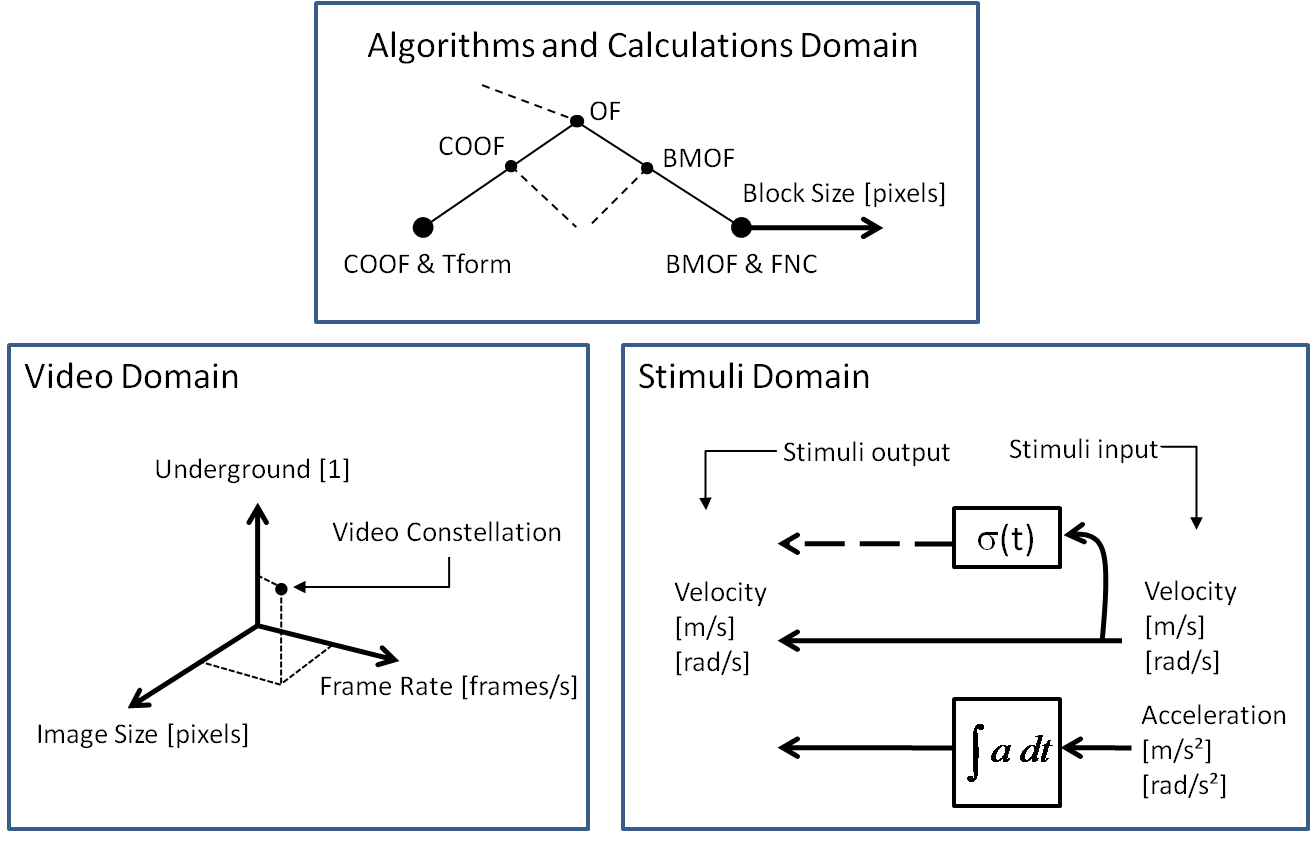
\includegraphics[width=1\textwidth]{graphic/ImageProcessingAnalysisDomains.png}
	\caption{Image processing analysis domains in focus of this project}
	\label{fig:ImageProcessingAnalysisDomains.png}
\end{figure}

Finally, the regarded aspects in relation to this project of the video source behaviour are summarised in the video domain. To provide a realistic environment, the chosen ranges of experimental analysis are derived from the data-sheets and publications 
\footnote{See \citeref[p.35]{Ahr08}, \citeref[p.6]{BloWeiScaSie10},
\citeref[p.22]{Tip08}, \citeref{MIC06}, \citeref[p.4]{StoBaiHayMil09}}, presented in \ref{fig:CameraExamples.pdf}. Afterwards, the components and their corresponding decision criteria of the video domain are presented and discussed in the following points.



\begin{figure}[H]
	\centering
		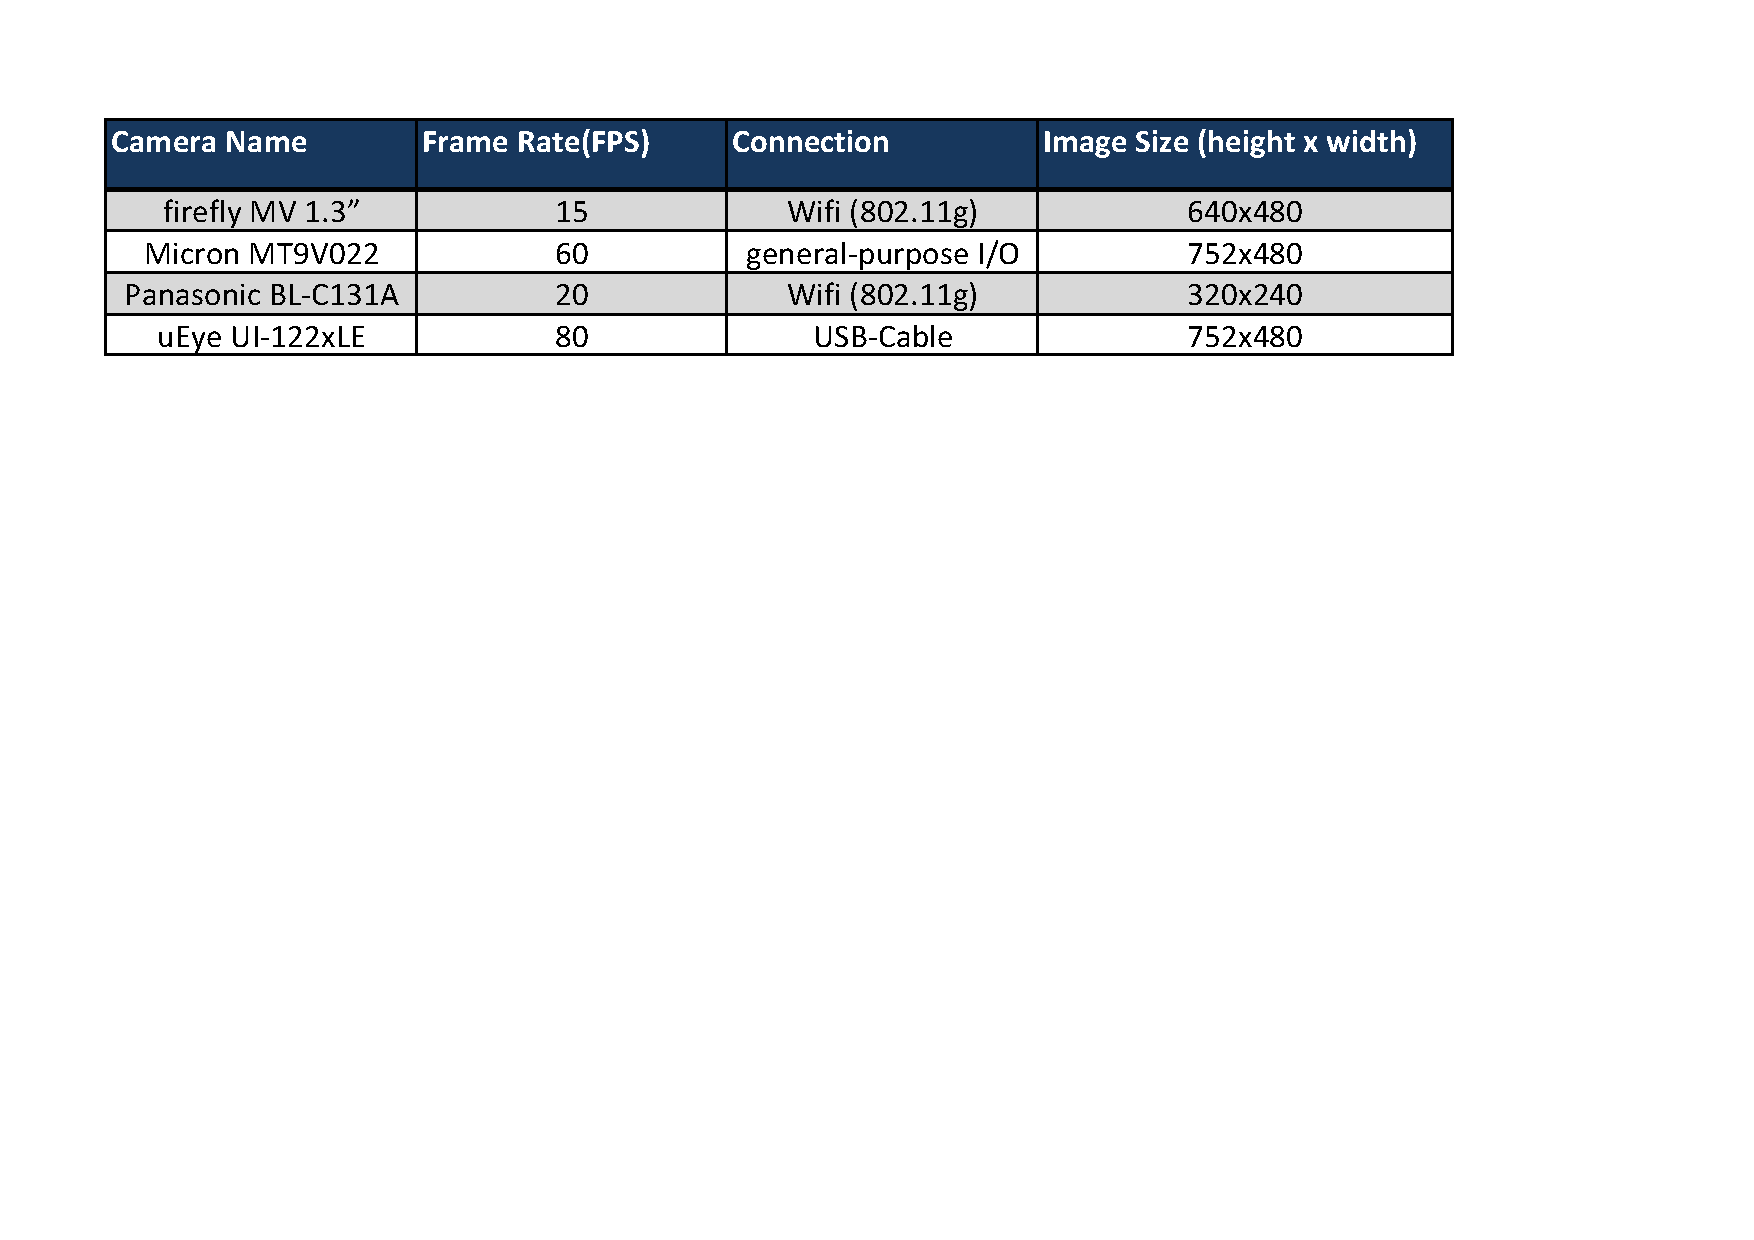
\includegraphics[width=1\textwidth]{graphic/CameraExamples.pdf}
	\caption{Examples of camera configurations derived from literature}
	\label{fig:CameraExamples.pdf}
\end{figure}

%\begin{table}
%\caption{\label{fig:CameraExmaples} Camera examples derived from literature}
%\begin{tabular}{|p{5cm}|p{1cm}|p{4cm}|p{2.5cm}|}
%\hline
 %Camera Name & FPS & Connection & Image Size\\
%\hline
%\hline
 %firefly MV 1.3'' & 15 & Wifi (802.11g) & 640x480\\
%\hline
 %Micron MT9V022 CMOS & 60 & general-purpose I/O & 752x480\\
%\hline
 %Panasonic BL-C131A & 20  & Wifi (802.11g) & 320x240\\ 
%\hline
%uEye UI-122xLE & 80 & USB-Cable & 752x480 \\
%\hline
%\end{tabular}
%\end{table}

\begin{itemize}

\item \textbf{Frame Rate}:

The frame rate is related to the maximum velocity in the regarded \gls{DOF}, which can be detected by the camera system.
 In relation to the image size, algorithm and calculation and the stimulus, it can be determined which constellation to the \gls{FPS} can provide satisfactory results. Generally, the ideal constellation is, regarding the frame rate, to reduce the processed images per second as far as possible. By doing this, the calculations, as well as the transmission complexity from quadrocopter to base-station, are reduced.
The variations which will be executed here in the experimental analysis are 10, 20, 40, 60, 80 FPS.

\item \textbf{Image Size}:
 
Similar to the frame rate, the image size can also influence the maximum velocity that can be detected by the camera system. Important thereby is the behaviour of the objects, moving relative to the camera system. Similarly, a big image window size allows to observe a bigger amount of points similarly. Furthermore, in a constellation of similar conditions, points are projected to a big image window for a longer period. In contrast to that, points stay into the focus of a small image for a short-time interval. Therefore, in such cases a higher image processing sample rate is desired to provide the same quality of results. On the other hand, if we also assume the same conditions of image composition, a bigger image window size requires a higher data size which also influences the transmission and the calculation of the image processing. Based on the camera examples presented in \ref{fig:CameraExamples.pdf}, the following image size variations in the corresponding experiments are 
320x240, 640x480, 768x576, 800x600, 1024x768 [height x width]. 

\item \textbf{Underground}:

The underground variation is a special behaviour of the experimental analysis related to this project. Based on the fact that the presented algorithms of optical movement detection focus different aspects of the image, it can be assumed that the motion detection behaviour will be alternating by varying undergrounds. So the undergrounds presented here focus two characteristics. As visualised in 
\ref{fig:Undergrounds.png}, the first underground (amorphous) provides amorphous groups of different contrasts. In contrast to that the second 
(segmented amorphous) provides additionally segmentations like edges and corners. Finally, the third (cornered) has mainly a cornered and edged structure. This variation of amorphous and corned structures provides a challenge to the algorithms that work with corner detection and block matching. 

\end{itemize}

\begin{figure}[H]
	\centering
		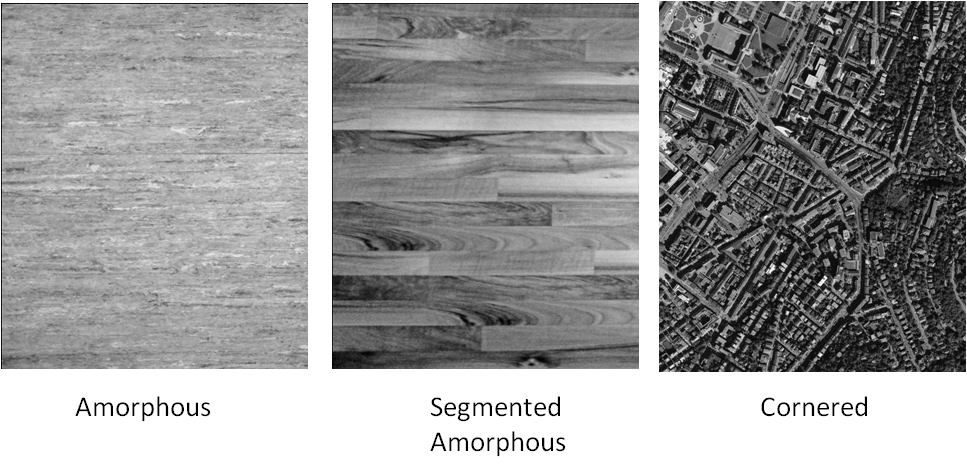
\includegraphics[width=1\textwidth]{graphic/Undergrounds.png}
	\caption{Different undergrounds with amorphous, segmented amorphous and cornered structure}
	\label{fig:Undergrounds.png}
\end{figure}

\subsection{Aspects of Reproducibility and Reliability}
\label{mt:c:expResults:ReproducibilityReliability}
This chapter introduces the methods executed to proof the correct function of the image processing simulation.
First, the sources which influence the test scenarios were analysed and evaluated. Thereby, it is important to clarify if there
are any elements inside these that generate noisy or randomly values. In case of the real and synthetic video source, this is not the case, because the 
real video never changes in the course of execution, and the synthetic video generates the same output with the corresponding same input.
To verify this reproducibility, and further the correctness of the synthetic video, two experiments were executed several times. These experiments are visualised in figure \ref{fig:SyntheticVideoEvaluation.png}. As shown, a special underground for measuring the movement is installed for the rotational and translational test. Furthermore, the movements \ensuremath{\Delta \psi}, \ensuremath{\Delta x} and 
\ensuremath{\Delta y} are tested versus the corresponding simulation time \ensuremath{\Delta t}. The result can be compared with the configured stimulus, and it can also be evaluated whether the velocity input was realised correctly. These test case executions show that the synthetic video environment is reliable and reproducible.

\begin{figure}[H]
	\centering
		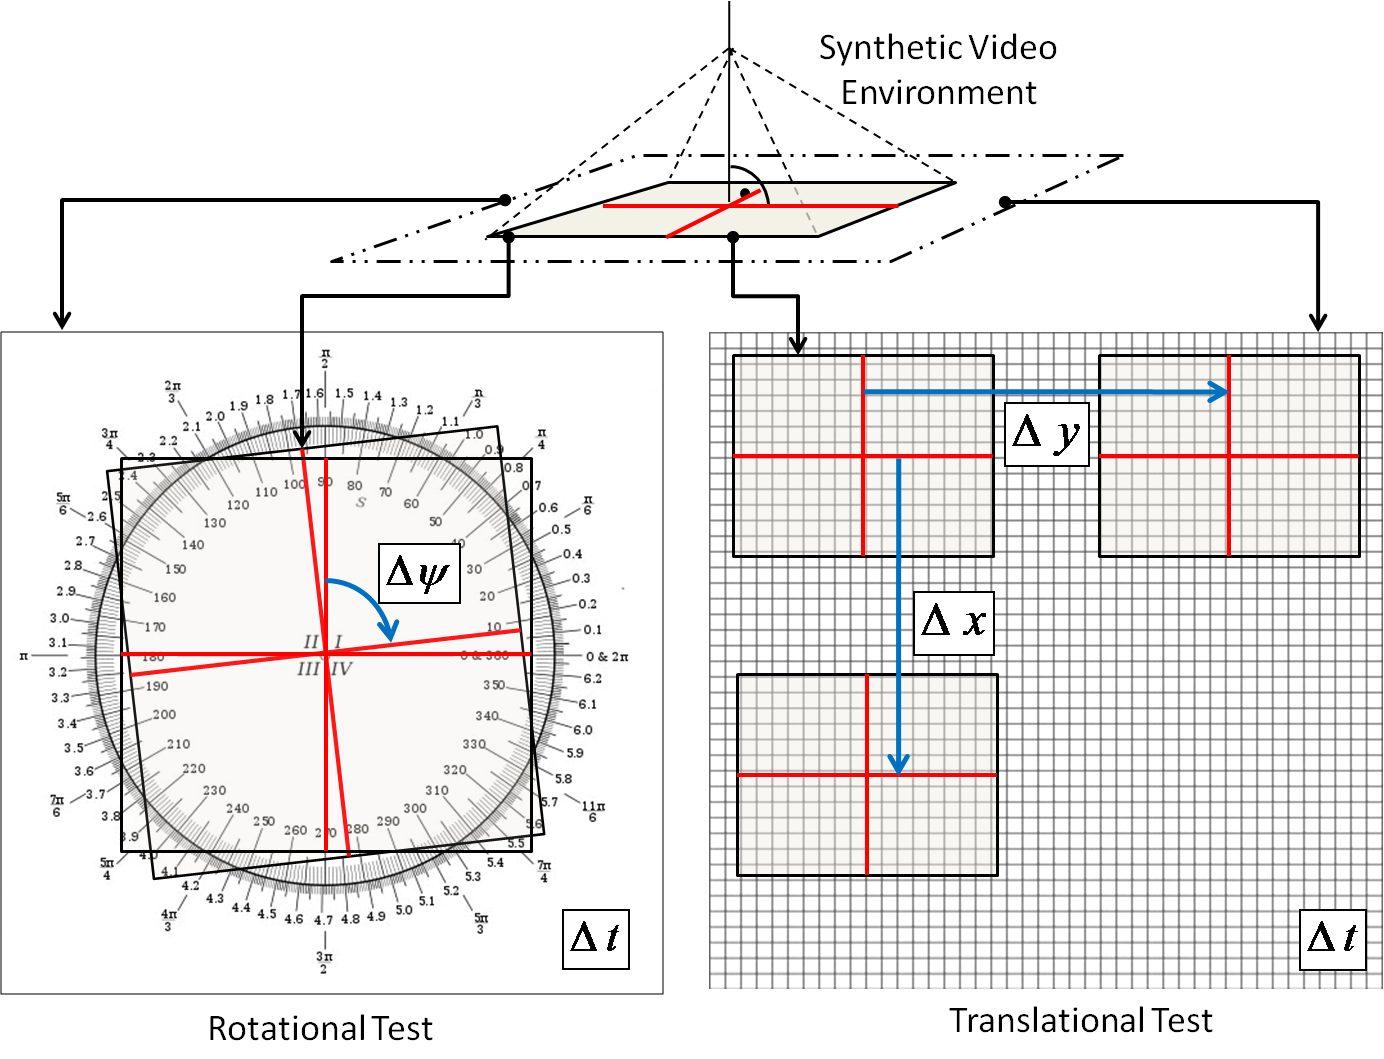
\includegraphics[width=1\textwidth]{graphic/SyntheticVideoEvaluation.png}
	\caption{Evaluation of Synthetic Video}
	\label{fig:SyntheticVideoEvaluation.png}
\end{figure}


%\section{Limits of simulation environment}
%\label{mt:c:expResults:AnalysisofImageProcessing:LimitsofSimulationenvironment}
%
%%Noise cannot exist in this case in the reality. That means the noise of the diagrams shows always inside the sample steps noise behaviour. The reason for that could be that the algorithm simulation calculates the same sequence of images multiple times in a single step.
%%BMOF Algorithm is possibly not robust against offset errors. That means that each customisation of the  block size needs a special investigation of offset errors. This equalisation is not realised inside the BMOF algorithm.
%
%%Show the calibration experiments and proof
%%Say why the experiments are reproducible


\subsection{Test Scenarios, Expectations and Results}
As presented in figure \ref{fig:ImageProcessingAnalysisDomains.png}, the variance rate is enormous. So the optical movement detection algorithms and corresponding calculations are tested in several scenarios which focus a specific behaviour with a corresponding expectation of the result. The goal thereby is to provoke expected characteristics, or to demonstrate that the expectations are not fulfilled by the result of the corresponding test scenario. For a better overview, the test plan \ref{fig:TestPlanOpticalFlow.png} shows the relations between the domains of variation. Each scenario is driven by a stimulus data which contains the three mentioned components of the stimuli domain, presented in 
\ref{fig:ImageProcessingAnalysisDomains.png}. Beside this, each test scenario separately focuses on the rotational and translational behaviour. 

\begin{figure}[H]
	\centering
		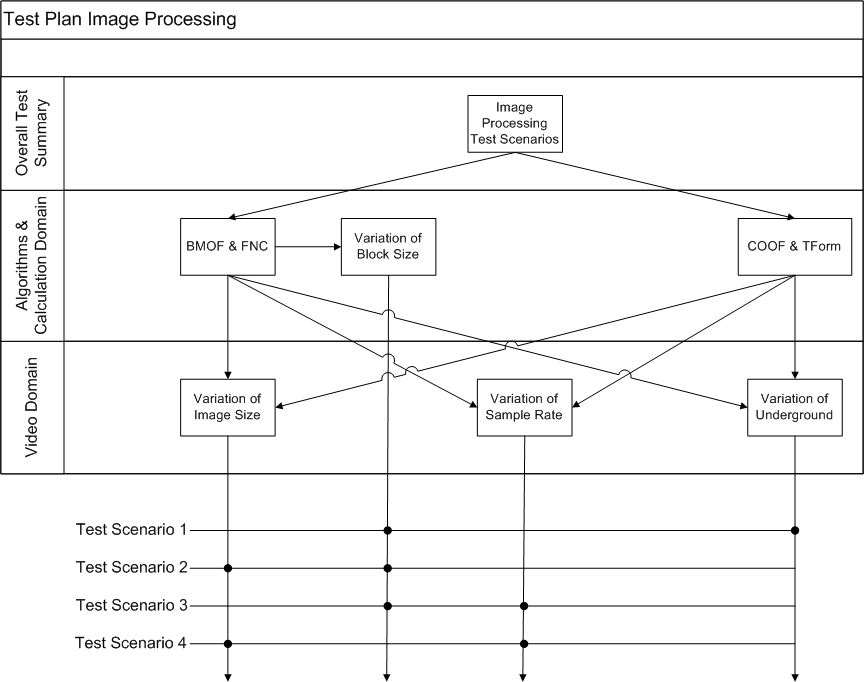
\includegraphics[width=1\textwidth]{graphic/TestPlanOpticalFlow.png}
	\caption{Image Processing Test Plan}
	\label{fig:TestPlanOpticalFlow.png}
\end{figure}

\subsubsection{Image Processing Test Scenario 1: Variation of Underground}
As mentioned in the description of the underground item, a flight scenario can be influenced by the underlying underground image. So this test scenario focused on the behaviour of the different algorithms in relation to the underground. To provide suitable results for investigation, the configurations of the used algorithms must also been varied. In this case, it is interesting to vary the \gls{BMOF} algorithm's block size, which can have an impact on the result.
This scenario bases on the expectation that the structure of the underground influences the quality of movement detection in relation to the used algorithm. Furthermore, as expected, the \gls{COOF} algorithm should show the best results on the cornered underground, because the built-in corner tracker can find a bigger amount of features. On the other hand, the \gls{BMOF} should operate satisfactory in the amorphous structure. The reason for this expectation is that the similarity measure of blocks is not as high as in the corned structure, because of the amorphous behaviour. This measure should influence the rate of exactly matching blocks. Finally, the segmented amorphous structure should expectably demonstrate that both algorithms work moderate on this structure, but not as good as in the expected more advantageous structure.

\subsubsection{Image Processing Results of Test Scenario 1}
Starting with the translational analysis of test scenario 1, the result presented in \ref{fig:Eval_IP_TS1_1.png} shows the characteristic of the \gls{COOF} algorithm. The expected best case behaviour for this algorithm is proved to be as expected, the cornered structure. Interesting to see is that the segmented amorphous underground nearly shows the same results as the best case. The amorphous underground affects, as expected, some outlines (See \ref{fig:Eval_IP_TS1_1.png} arrow No.2), probably because the found feature amount is not high enough, or some features raise errors because of the same structure. On the other hand, this assumption could be the reason for the apparent better detection ability of the acceleration stimulus part with the cornered structure (See \ref{fig:Eval_IP_TS1_1.png} arrow No.4). Another unexpected behaviour, which is probably related to the sample time, is that the complete output curves react with a delay of 100ms 
(See \ref{fig:Eval_IP_TS1_1.png} arrow Nr.1 and Nr.3).          

\begin{figure}[H]
	\centering
		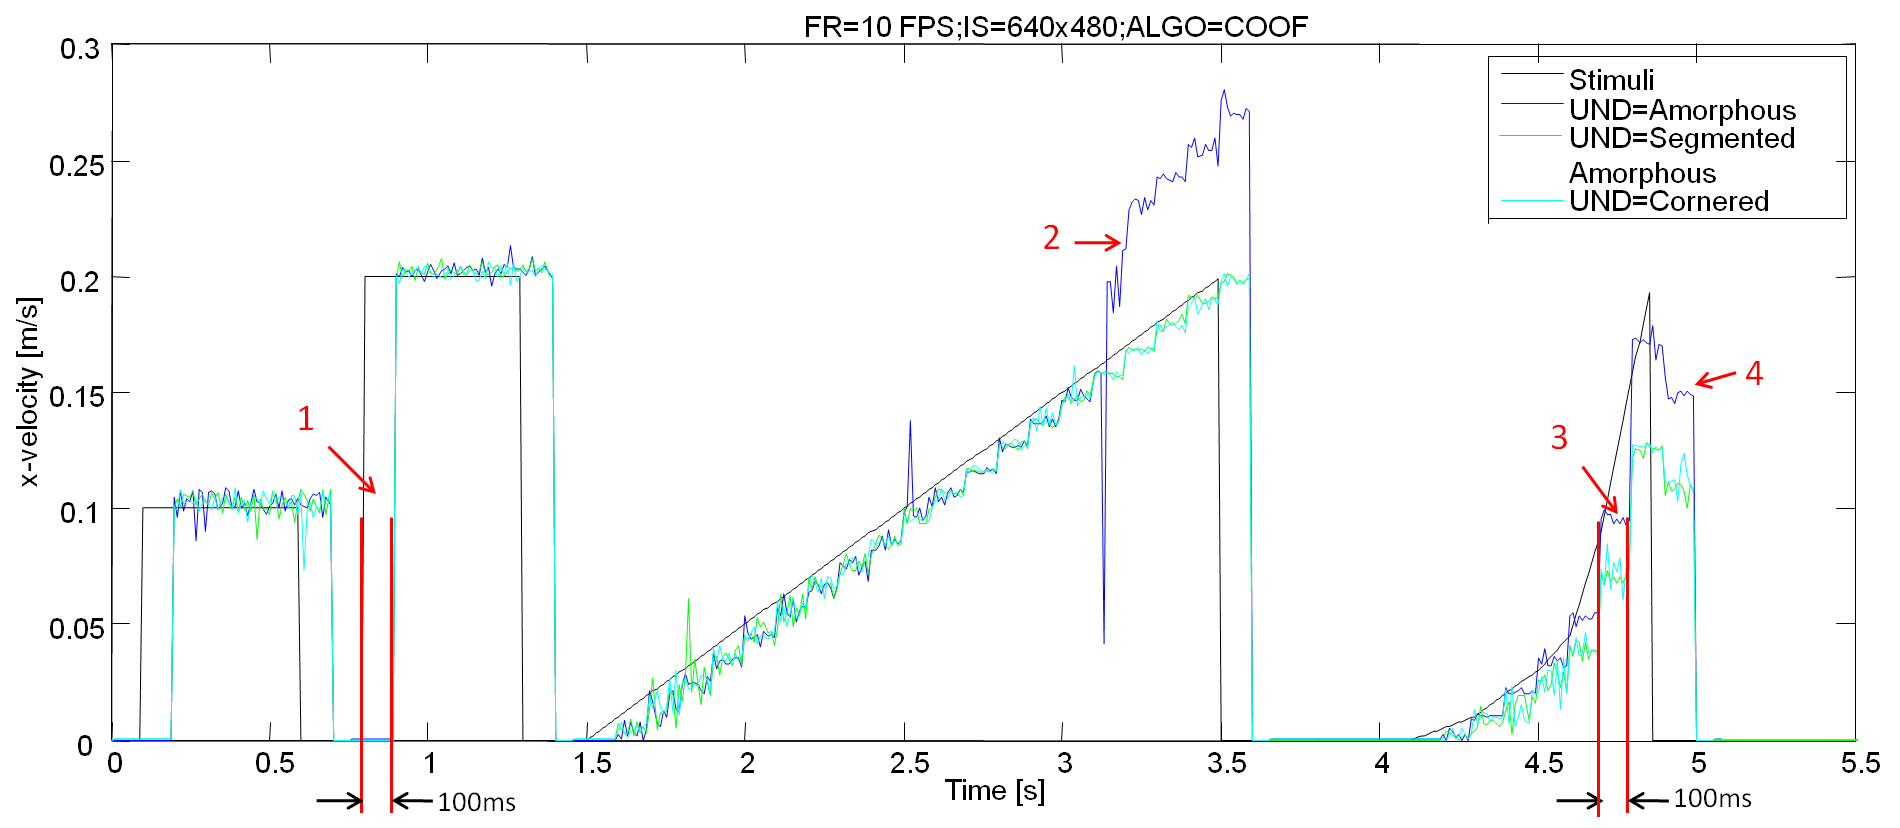
\includegraphics[width=0.95\textwidth]{graphic/Eval_IP_TS1_1.png}
	\caption{Image Processing Result of Test Scenario 1: Translational analysis of COOF}
	\label{fig:Eval_IP_TS1_1.png}
\end{figure}

The results of the \gls{BMOF} algorithm are visualised in figure \ref{fig:Eval_IP_TS1_2.png}. Thereby the unexpected but interesting behaviour was found that the \gls{BMOF} algorithm reaches the limit of maximum velocity, in this special case \ensuremath{0.1 m/s}, faster as the \gls{COOF} algorithm under equal conditions. Furthermore, the expected best suited underground is the amorphous structure, but just on the aspect of precision (See arrows No.1, \ref{fig:Eval_IP_TS1_2.png}). But this noise behaviour could also be a limitation of the simulation, caused by multiple calculations of the same sampled image sequence (See arrow No.2 and No.3). Another unexpected behaviour is that the \gls{BMOF} algorithm has a better offset behaviour, in relation to its block size, with the cornered structure.
This means that the \gls{BMOF} algorithm does not normalise the detected velocities in relation to the blocks, to a relative level that affects the problem that a coarse-grained block segmentation has a lower offset in the equal environment as a fine-grained segmentation.

%\begin{figure}[H]
	%\centering
		%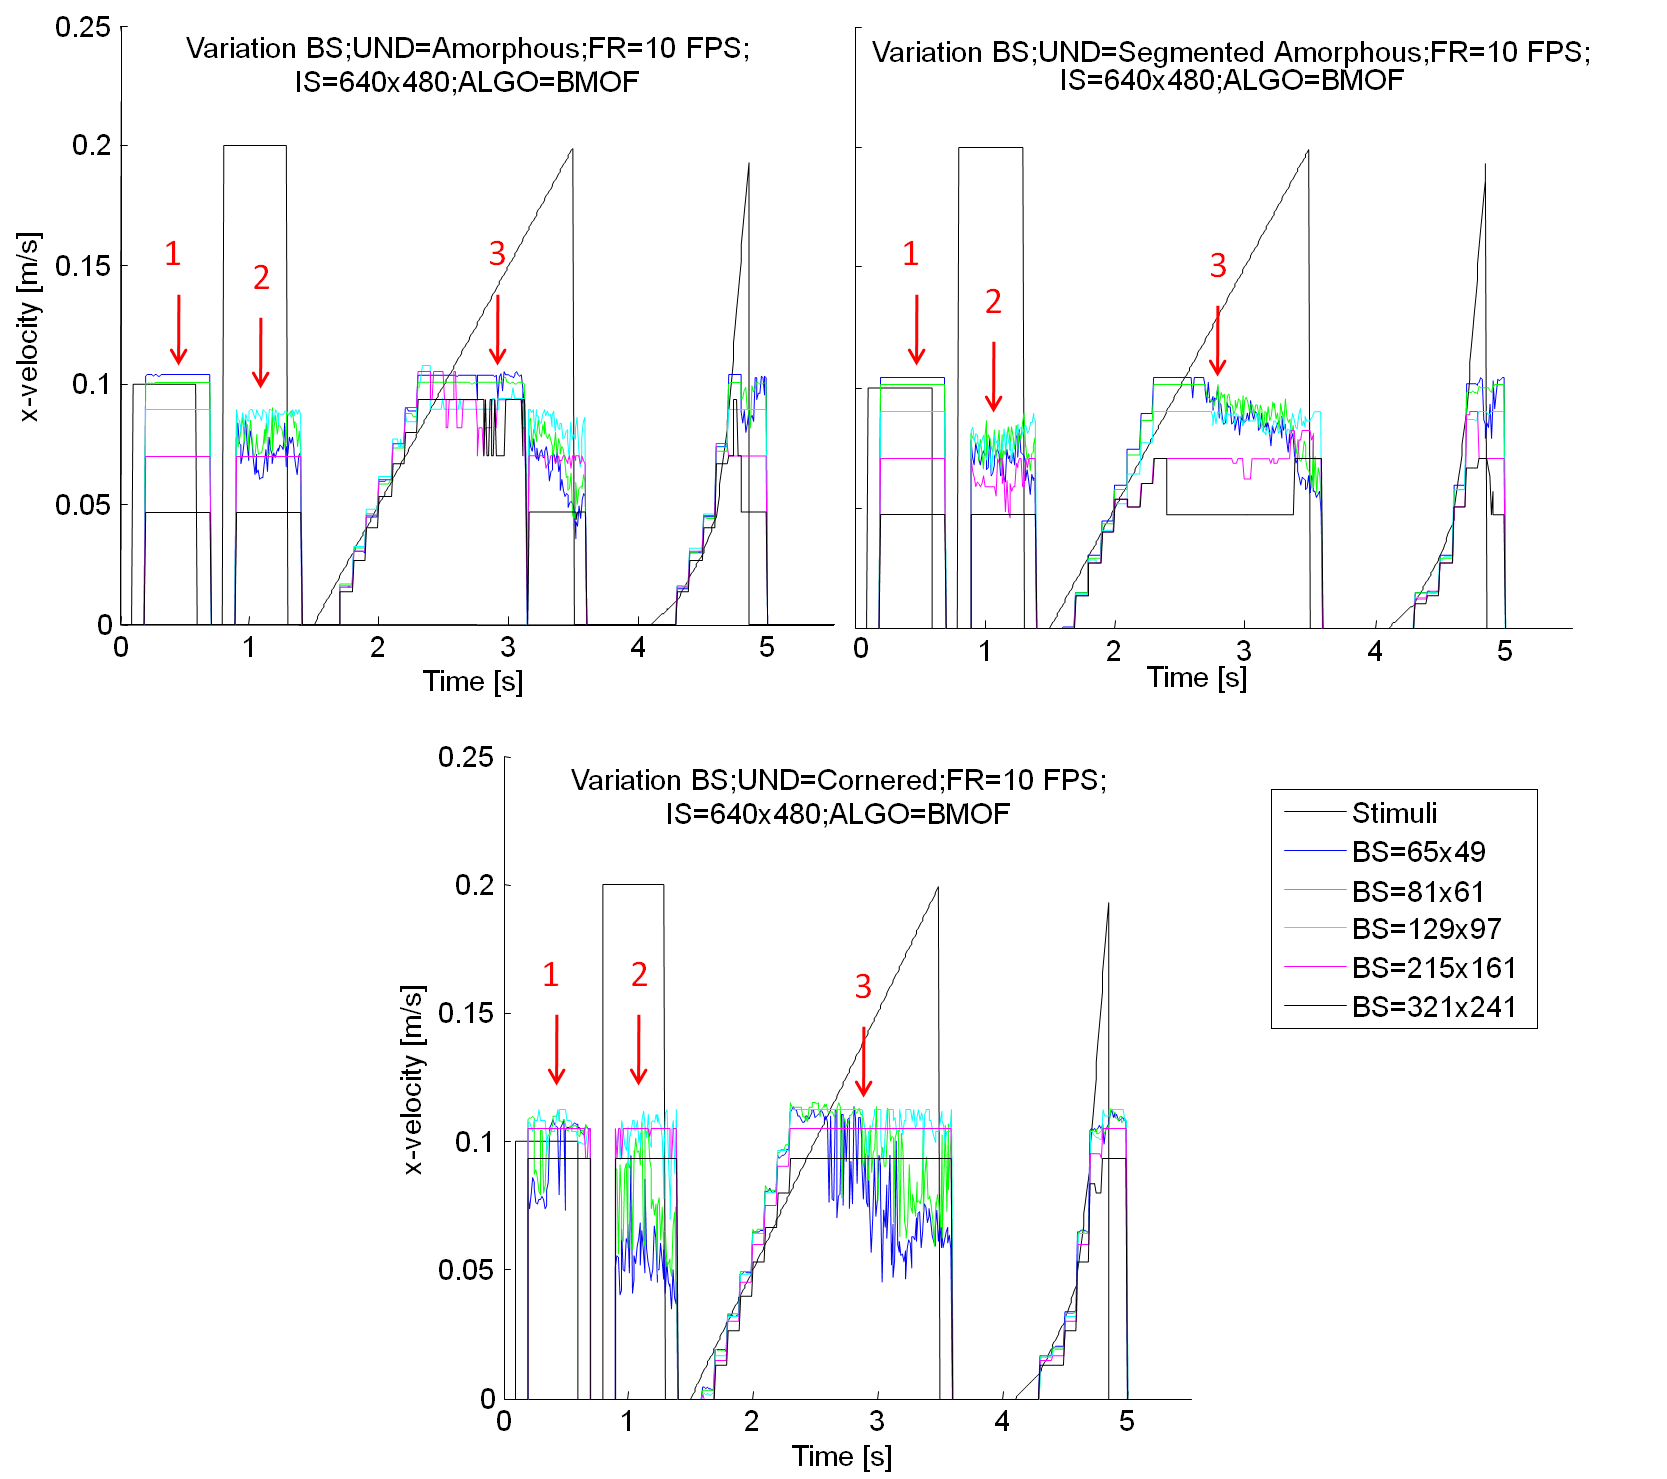
\includegraphics[width=1\textwidth]{graphic/Eval_IP_TS1_2.png}
	%\caption{Result of Test Scenario 1: Translational analysis of BMOF}
	%\label{fig:Eval_IP_TS1_2.png}
%\end{figure}

\begin{figure}[H]
\subfigure[]{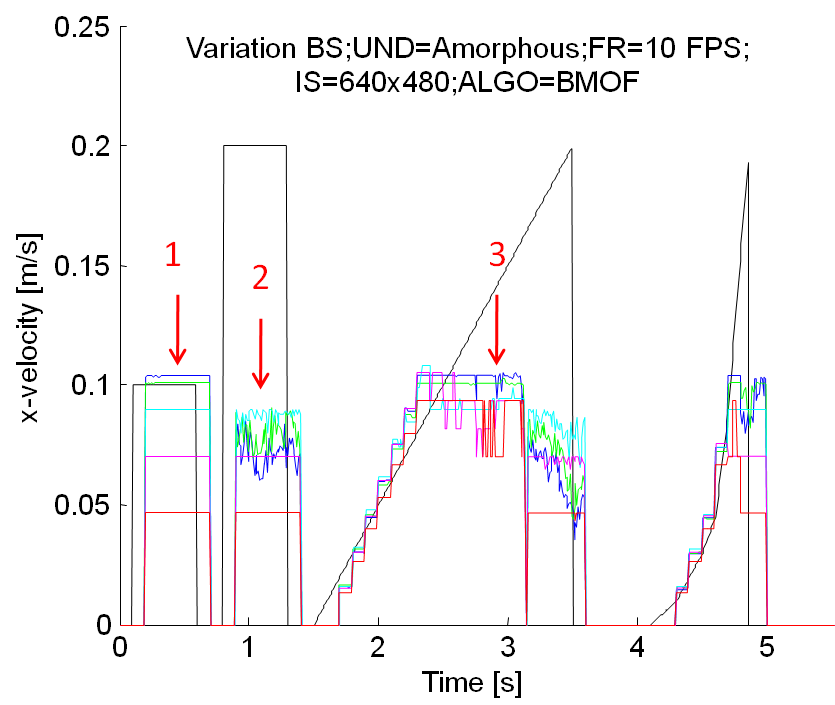
\includegraphics[width=0.50\textwidth]{graphic/Eval_IP_TS1_2_a.png}}\hfill
\subfigure[]{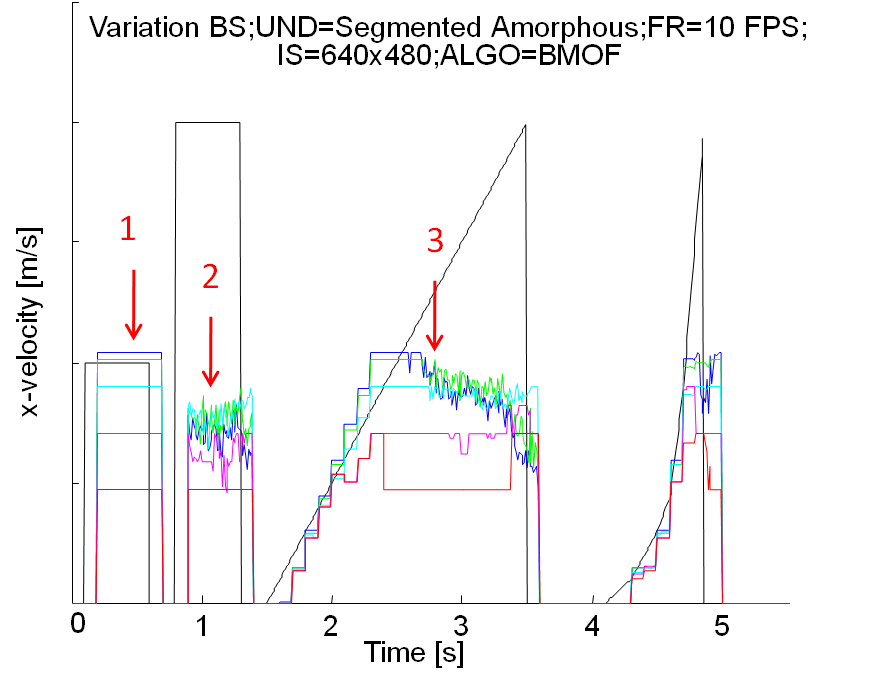
\includegraphics[width=0.50\textwidth]{graphic/Eval_IP_TS1_2_b.png}}
\begin{center}
\subfigure[]{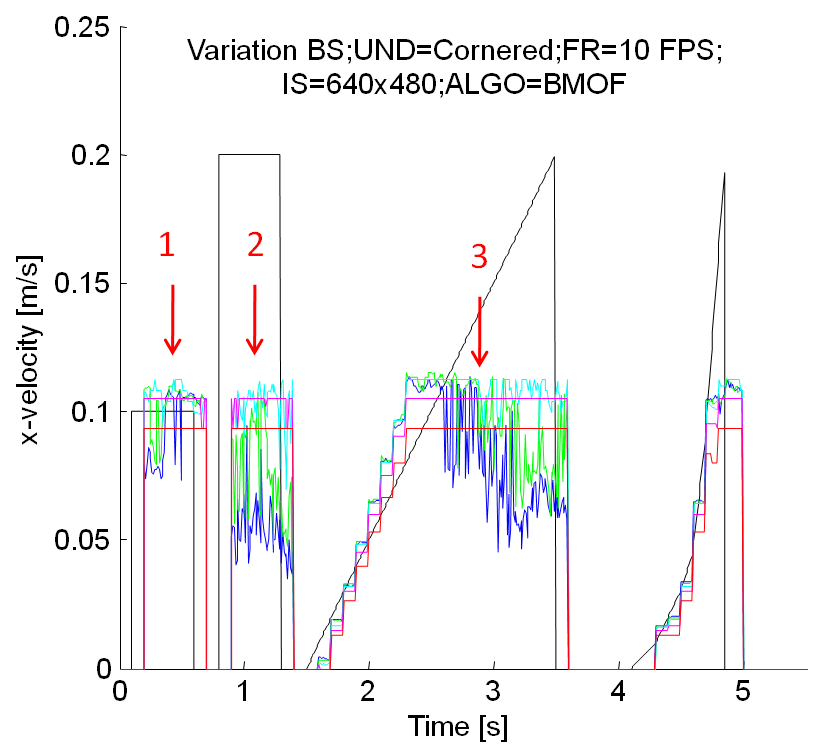
\includegraphics[width=0.50\textwidth]{graphic/Eval_IP_TS1_2_c.png}}
\end{center}
\begin{center}
\subfigure{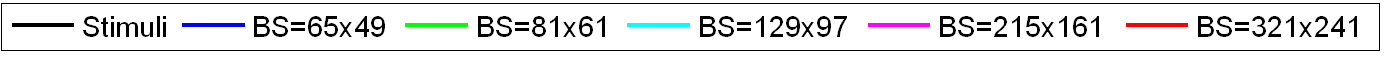
\includegraphics[width=1\textwidth]{graphic/Eval_IP_TS1_2_legend.png}}
\end{center}
\caption{Image Processing Result of Test Scenario 1: Translational analysis of BMOF}
\label{fig:Eval_IP_TS1_2.png}
\end{figure}

Afterwards, the experimental results of the rotational behaviours show enormous differences in several aspects. First, the diagram (a) in
figure \ref{fig:Eval_IP_TS1_3.png} visualises the rotational \gls{COOF} algorithm behaviour in a test with a maximum gain of 
 \ensuremath{2*\pi/s}. As mentioned, the \gls{COOF} algorithm can detect the rotational direction. This information is reflected in the sign of the detected velocity. As visualised, the negative direction of the rotational behaviour shows a counter-clockwise rotation. As we can see, the first pulse, with a gain of \ensuremath{\pi} is nearly error-free detected (See \ref{fig:Eval_IP_TS1_3.png} arrow No.1). In contrast to that, the \gls{COOF} algorithm shows problems with reaching the gain of \ensuremath{2*\pi}, 
(See \ref{fig:Eval_IP_TS1_3.png} arrows No.2 and No.3). These errors are possibly based on the combination of a rotational movement and the low sample rate. Such an effect is also discussed and presented in the stroboscopic torque measurement in chapter 
\ref{mt:c:design:Analysis of Existing Quadrocopter Architecture:Characteristics of Sensors and Actuators}. Unexpected was in this case that the \gls{COOF} algorithm also showed errors with the amorphous and cornered structure, but provides the best matches with the segmented amorphous structure. The reason could be a big amount of dissimilar forms, based on the amorphous and cornered structure. 
The diagram (b) shows the result of the \gls{BMOF} algorithm, which is under no circumstances useful. In this case, it is obvious that the low sample rate along with the corresponding hight rotational velocity affects a big amount of error matchings.

%\begin{figure}[H]
	%\centering
		%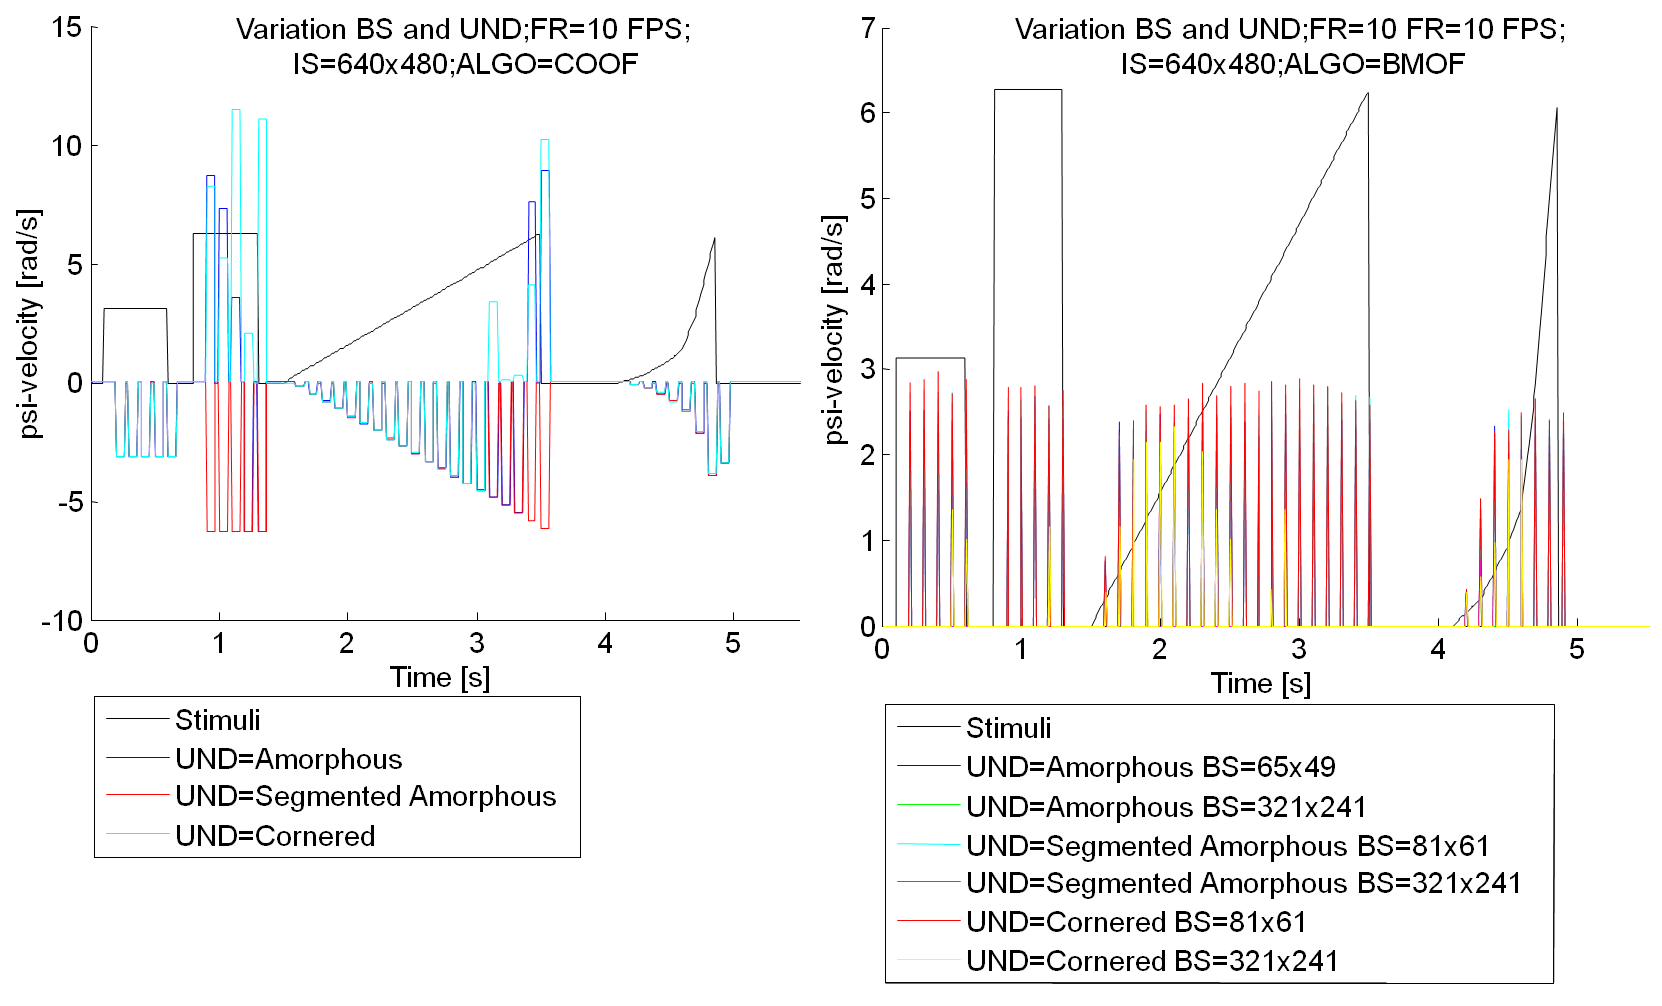
\includegraphics[width=1\textwidth]{graphic/Eval_IP_TS1_3.png}
	%\caption{Result of Test Scenario 1: Rotational analysis of BMOF and COOF}
	%\label{fig:Eval_IP_TS1_3.png}
%\end{figure}

\begin{figure}[H]
	\subfigure[]{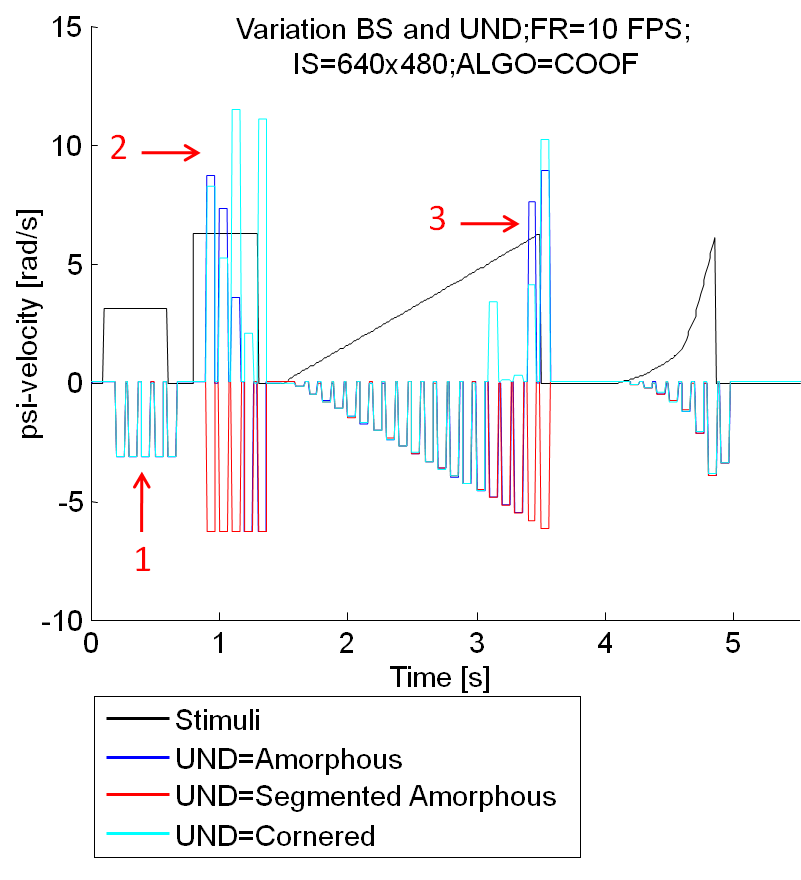
\includegraphics[width=0.50\textwidth]{graphic/Eval_IP_TS1_3_a.png}}\hfill
	\subfigure[]{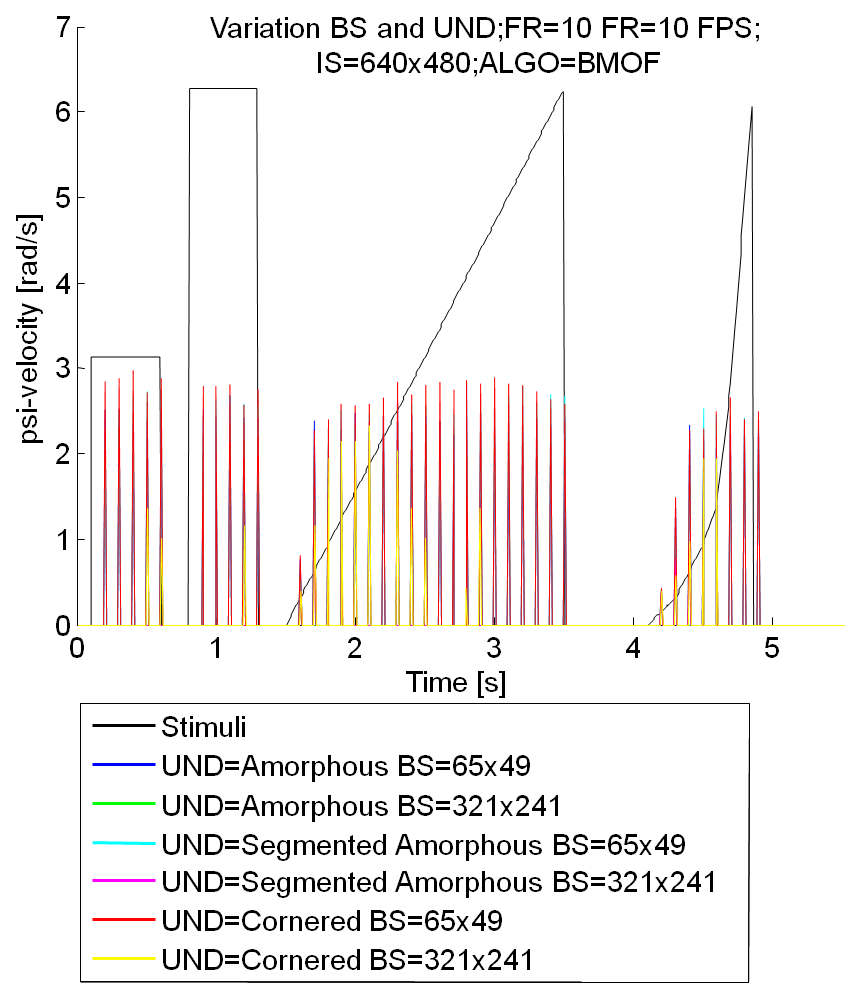
\includegraphics[width=0.50\textwidth]{graphic/Eval_IP_TS1_3_b.png}}
	\caption{Image Processing Result of Test Scenario 1: Rotational analysis of BMOF and COOF}
	\label{fig:Eval_IP_TS1_3.png}
\end{figure}


Because of the poor rotational behaviour of the \gls{BMOF}, the rotational experiment of this algorithm was executed with a sample rate of 80 \gls{FPS}. The result is the first satisfactory configuration for the rotational behaviour of this algorithm. Returning to the original focus of this test scenario, the underground structure that showed the best results is the segmented amorphous with the fine-grained configuration of blocks (See \ref{fig:Eval_IP_TS1_4.png} arrow No.1). This behaviour is argumentative, because it acts like the \gls{COOF} algorithm. Possibly the mentioned reason of the highest dissimilarity of forms can also lie in the characteristic of best matches.

\begin{figure}[H]
	\centering
		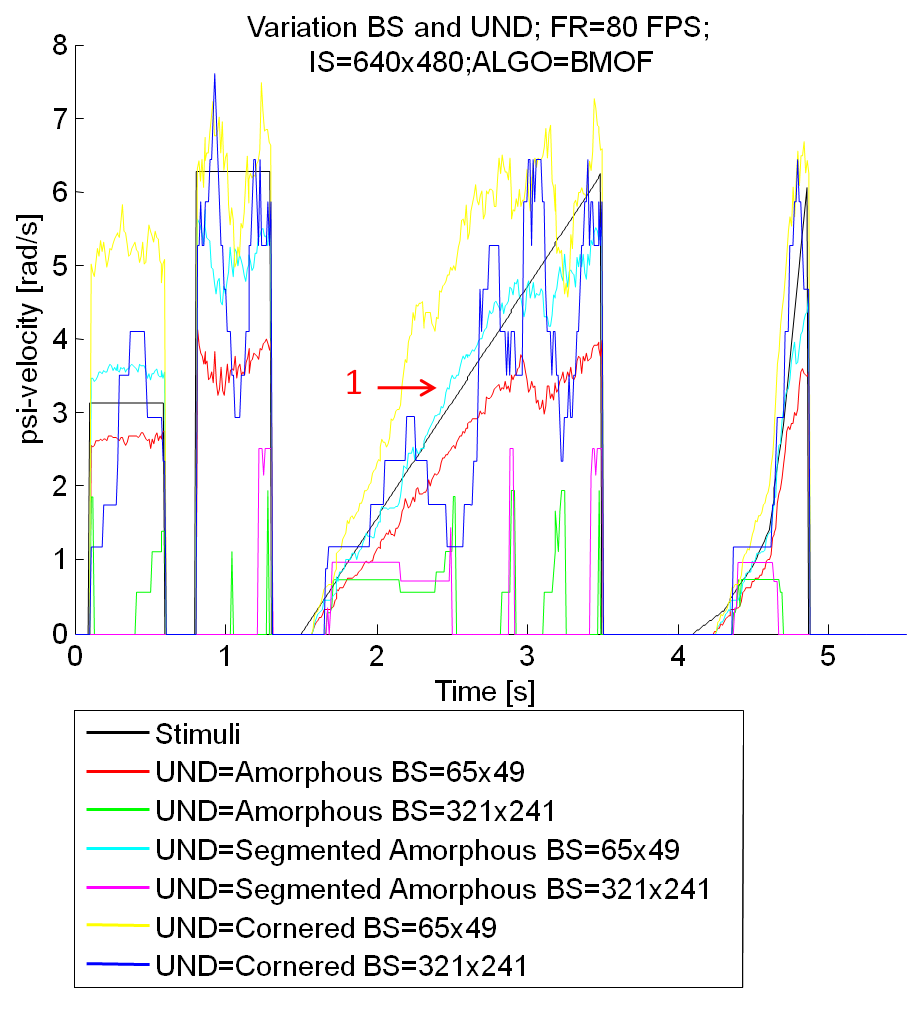
\includegraphics[width=0.70\textwidth]{graphic/Eval_IP_TS1_4.png}
	\caption{Image Processing Result of Test Scenario 1: Rotational analysis of BMOF with conformed frame rate}
	\label{fig:Eval_IP_TS1_4.png}
\end{figure}

\subsubsection{Image Processing Test Scenario 2: Variation of Image Size}
The image size of the captured images is related to this data size, and further to the transmission time to the base station. So this test sequence focuses on the variation of usual image sizes, presented in the introduction of this chapter and based on the presented camera examples in 
\ref{fig:CameraExamples.pdf}. As is well known from the first test scenario, the block size of the \gls{BMOF} is also being varied in this test case to analyse the corresponding relation of block and image size. The underground which was chosen in this scenario is the segmented amorphous structure, which was not changed over the test execution.
The goal and expectation of this test case is to demonstrate the relation of image size and maximum translational or rotational speed that can be detected. Also interesting is to investigate whether the precision of movement detection is related to the image size. This expectation is based on the assumption that more points can be captured in a bigger image and this leads to a more exact determination of movement.
Another interesting characteristic is the question which algorithm can provide a better performance in aspects of precision and maximum speed with the same image size. The expectation is that the \gls{COOF} algorithm will show better results and will not be as dependant on the image size, as the \gls{BMOF} algorithm. This assumption bases on the fact that \gls{COOF} takes all tracked features similarly into account in each step, and is not dependent on a limited search area as is the case with the \gls{BMOF} algorithm.

\subsubsection{Image Processing Results of Test Scenario 2}
The unsatisfactory result of the rotational behaviour of the \gls{BMOF}, presented in \ref{fig:Eval_IP_TS1_3.png} (b), lead to the decision to change the frame rate for test scenario 2. So the frame rate of this test scenario was increased form 10 \gls{FPS} to 80 \gls{FPS} for feasibility reasons. 
Starting with the \gls{BMOF} algorithm, the executed tests are visualised in \ref{fig:Eval_IP_TS2_1.png}. Thereby, diagram (a) contains the 
executed test scenario with the smallest block size (fine-grained), and diagram (b) presents the output of the algorithm with the biggest block size (coarse-grained). Generally, the drawback of the fine-grained configuration can be seen in the second pulse. In contrast to the coarse-grained configuration, the fine-grained output shows a noisy gain behaviour(\ref{fig:Eval_IP_TS2_1.png} (a) arrow No.1 ). Additionally, the fine-grained configuration shows the unexpected behaviour of more exactly reaching the stimulus signal in the ramp phase (\ref{fig:Eval_IP_TS2_1.png} (a) and (b) arrow No.2). Combined with the result that the fine-grained configuration is more noisy, it is logical that it reacts faster as the coarse-grained configuration. Regarding the small velocities of the ramp and exponential part of the stimulus, it is noticeable that all image size configurations have a small dead zone before they react to the stimulus (\ref{fig:Eval_IP_TS2_1.png} (a) and (b) arrow No.4). So because this characteristic exists in all configurations, and was not detected in test scenario 1, it is possible that it is related to the increased frame rate of this scenario.  
Furthermore, we can see that the maximum speed limit is not as much related to the image size in the configuration of this scenario as expected. This can be assumed because the difference in the output error between the biggest and smallest image size, with the best block size configuration, is less then 10\text{\%} (\ref{fig:Eval_IP_TS2_1.png} (a) and (b) arrow No.3).
A better visualisation of all test errors, executed in each constellation of block and image size, is visualised in diagram 
\ref{fig:Eval_IP_TS2_1.png} (d). As expected, the smallest image size corresponds to the biggest errors. Further, it is interesting to see that least errors are reached diagonal to the block and image size axis. This means that the optimal configuration is related to the optimal segmentation of the image with the corresponding block size (\ref{fig:Eval_IP_TS2_1.png} (d) blue concave area). 
The translational behaviour of the \gls{COOF} in relation to the image size is visualised in diagram \ref{fig:Eval_IP_TS2_1.png} (c). 
As anticipated, this algorithm shows nearly the same behaviour in each configuration of the image size. The unexpected behaviour is that the output signals' noise is bigger than in a similar test with a sample rate of 80 \gls{FPS}. So it can be assumed that the sample rate has a bigger impact on the noise and precision of the \gls{COOF} algorithm as the image size. 

\begin{figure}[H]
\subfigure[]{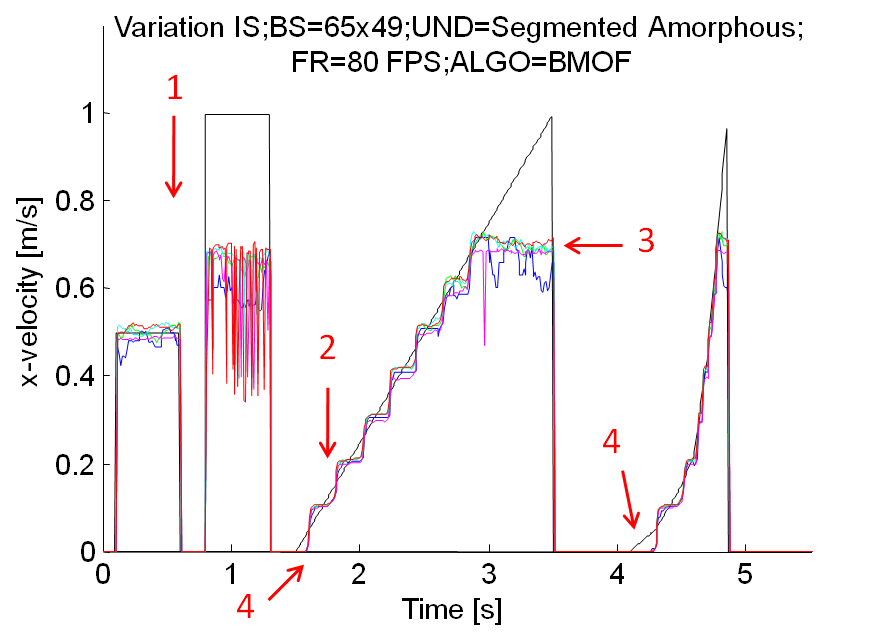
\includegraphics[width=0.50\textwidth]{graphic/Eval_IP_TS2_1_a.png}}\hfill
\subfigure[]{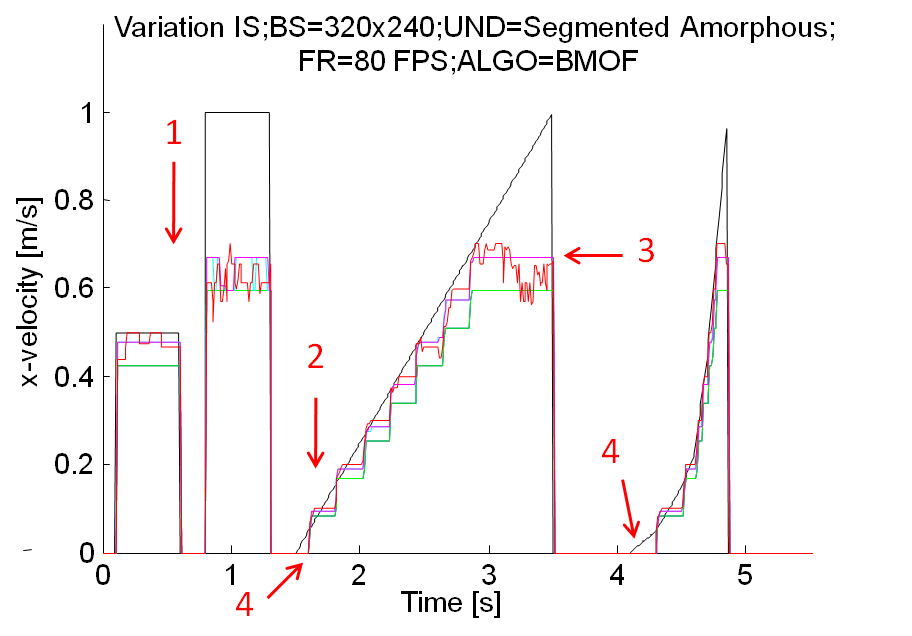
\includegraphics[width=0.50\textwidth]{graphic/Eval_IP_TS2_1_b.png}}
\subfigure[]{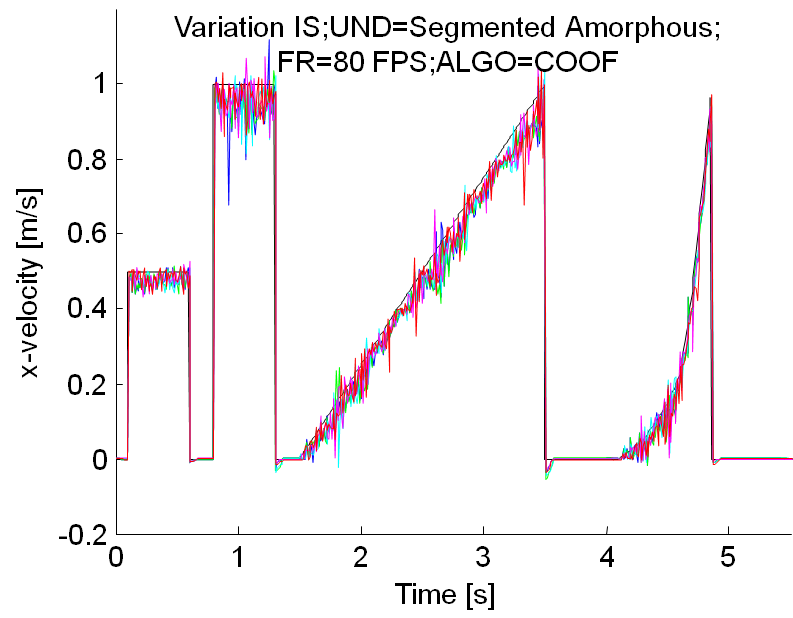
\includegraphics[width=0.50\textwidth]{graphic/Eval_IP_TS2_1_c.png}}
\subfigure[]{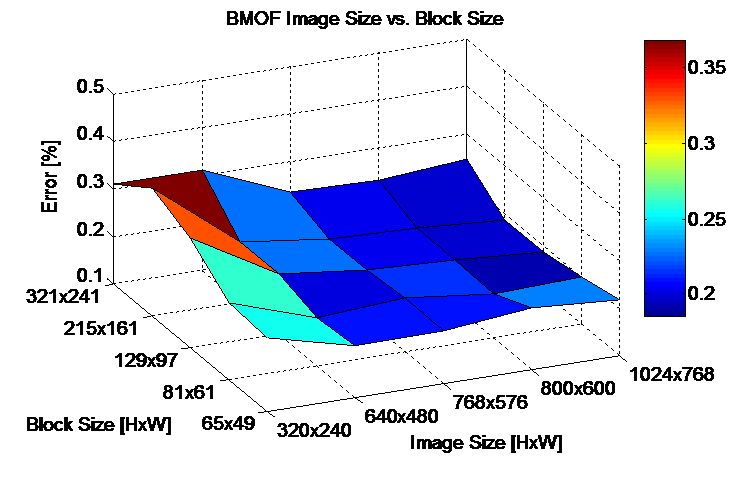
\includegraphics[width=0.50\textwidth]{graphic/Eval_IP_TS2_1_d.png}}
\begin{center}
\subfigure{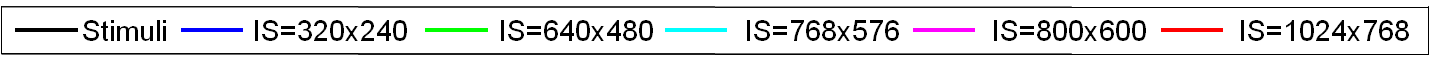
\includegraphics[width=1\textwidth]{graphic/Eval_IP_TS2_1_legend.png}}
\end{center}
\caption{Image Processing Result of Test Scenario 2: Translational analysis of BMOF and COOF}
\label{fig:Eval_IP_TS2_1.png}
\end{figure}

On closer consideration of the rotational result in relation to the image size, as expected the \gls{COOF} operates nearly perfectly in contrast to the \gls{BMOF}. As visualised in diagram \ref{fig:Eval_IP_TS2_2.png}(c), the test scenario with a maximum limit of \ensuremath{2 \pi / s} rotational velocity could not utilise the maximum limit of the algorithm. So this experiment was executed again with a higher gain, to reach and investigate the limitation of \gls{COOF}. The result is that the rotational velocity limits of the \gls{COOF} are nearly 
two times and the translational even five times higher than the best-suited configuration of \gls{BMOF}.
By regarding the fine-grained (a) and coarse-grained (b) block size rational behaviour of the \gls{BMOF}, it is interesting to see that the 
fine-grained configuration is superior to the coarse-grained. The unexpected behaviour thereby is that the best error value is reached with  corresponding middle or small image sizes (blue area in figure \ref{fig:Eval_IP_TS2_2.png}(d)) and not with the biggest image sizes. Thereby, this deviation is not that big, so it is possible that this phenomenon originates from the Gaussian distribution off errors, related to the underground. On the other hand, it is possible, as mentioned in the investigations of the translational behaviour, that an ideal configuration of image size and block size results in average from an error minimum. 
 
\begin{figure}[H]
\subfigure[]{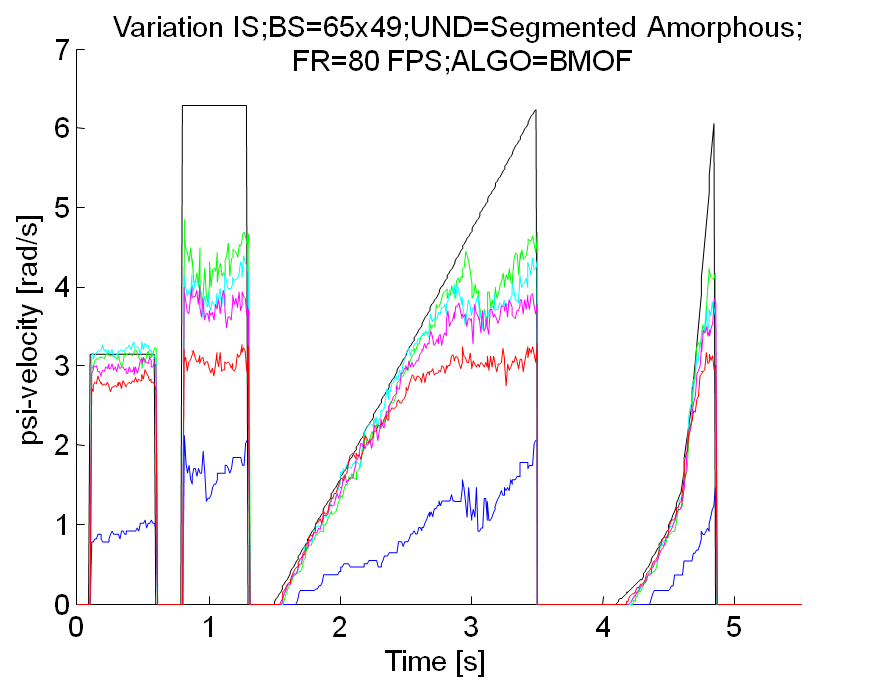
\includegraphics[width=0.50\textwidth]{graphic/Eval_IP_TS2_2_a.png}}\hfill
\subfigure[]{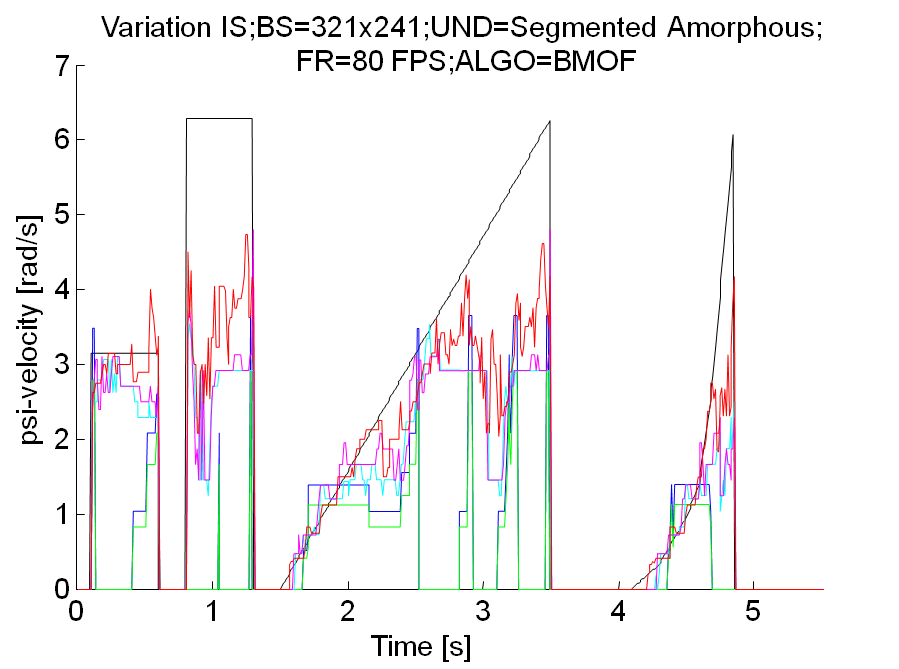
\includegraphics[width=0.50\textwidth]{graphic/Eval_IP_TS2_2_b.png}}
\subfigure[]{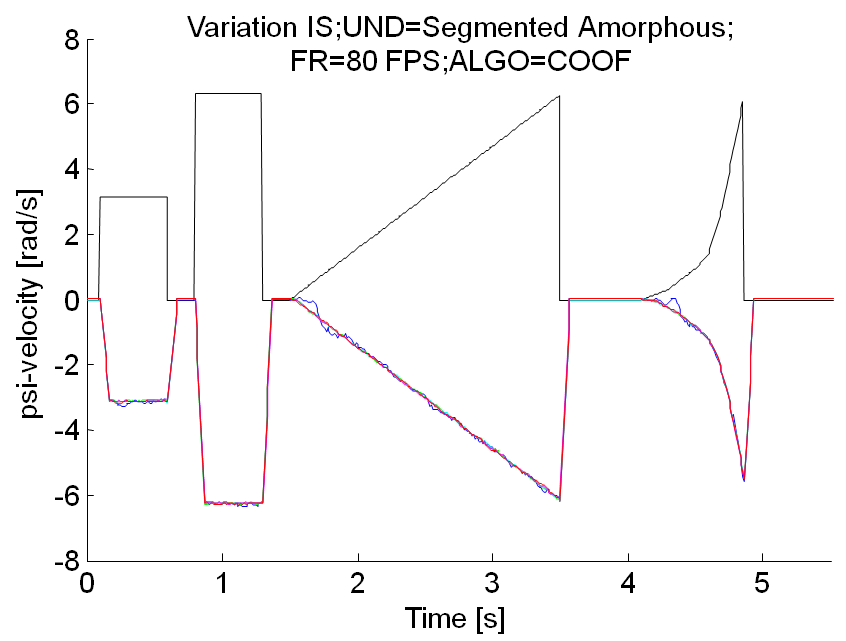
\includegraphics[width=0.50\textwidth]{graphic/Eval_IP_TS2_2_c.png}}
\subfigure[]{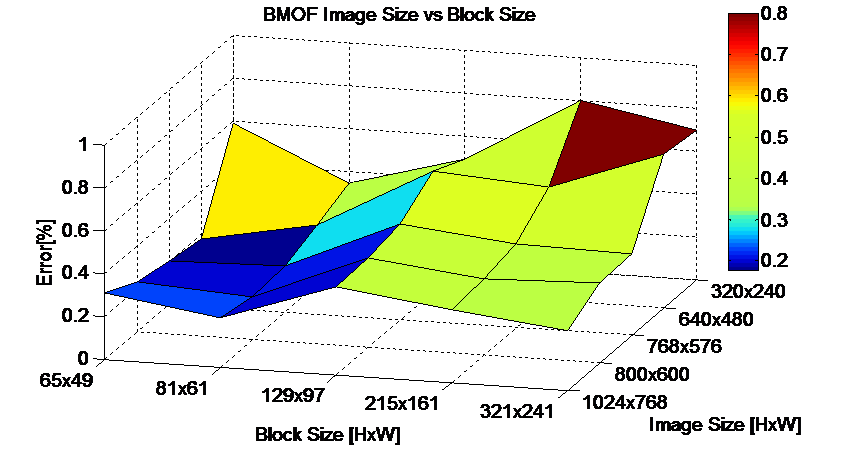
\includegraphics[width=0.50\textwidth]{graphic/Eval_IP_TS2_2_d.png}}
\begin{center}
\subfigure{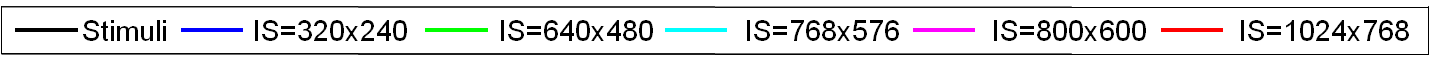
\includegraphics[width=1\textwidth]{graphic/Eval_IP_TS2_2_legend.png}}
\end{center}
\caption{Image Processing Result of Test Scenario 2: Rotational analysis of BMOF and COOF} 
\label{fig:Eval_IP_TS2_2.png}
\end{figure}


\subsubsection{Image Processing Test Scenario 3: Variation of Sample Rate}
The Sample Rate variation test scenario, based on MATLABS/Simulink's time variant simulation of dynamic systems, and provides the perspective to analyse the algorithm behaviour in relation to the presented rates in the introduction. As mentioned, similar to the image size, the frame rate also has an impact on the load factor of the image processing and transmission spectrum. So in this scenario, the introduced algorithms should be investigated with the intension to determine the limits of maximum speed operation, and to figure out which algorithm, with corresponding configuration, provides the best result related to the same frame rate. The expected result of this scenario is that both algorithms will reach a limit, but the \gls{COOF} will work with higher velocity conditions. Based on the mentioned expectation in test scenario 2, the limited search region of the \gls{BMOF} will increase the error possibility with ascending speed. On the other hand, the \gls{BMOF} algorithm should show a more precise processing at lower speed and frame rate, because with increasing successful block matches, the possibility of error matches is decreased. This expected characteristic could be demonstrated with a jigsaw puzzle example, in which also the possibility to find the right piece in a region increases in relation to the amount of already located pieces.  

\subsubsection{Image Processing Results of Test Scenario 3}
In the previous test scenarios, the rotational and translational speed limitation of \gls{BMOF}, related to the highest sample rate, was  determined and presented in \ref{fig:Eval_IP_TS2_2.png} (a) (b) and \ref{fig:Eval_IP_TS2_1.png} (a) (b). As expected, the \gls{COOF} algorithm shows better results in the aspect of speed limitation as \gls{BMOF}. The expected behaviour of higher precision in the region of a low sample rate of the \gls{BMOF} algorithm is shown in diagrams \ref{fig:Eval_IP_TS3_1.png} (a) and (b). As we can see, the fine-grained configuration shows a smoother characteristic of the output signal, in contrast to the coarse-grained block segmentation, which reacts step-wise to the stimulus. Unexpected thereby was that the highest sample rate has the biggest delays and reacts very quantitative in relation to stimulus change (\ref{fig:Eval_IP_TS3_1.png} (a) (b) arrow No. 2 and No.4). These delays, related to the ascending sample rate, could occur because the changes between the captured images are very small and could not be detected by the algorithm. That means velocity changes in the dead zone could remain undetected in a trajectory. On the other hand, sample rates over 20 \gls{FPS} can detect the stimulus signal up to the biggest velocity value. In contrast to that, the small sample rates 10 \gls{FPS} and 20 \gls{FPS} reach their limits in the presented diagrams 
(\ref{fig:Eval_IP_TS3_1.png} (a) (b) arrow No.3). As mentioned, the \gls{COOF} algorithm shows, with ascending sample rate, an ascending noise characteristic which could also originate from the small changes between the images, which rise to error localisations of the features (\ref{fig:Eval_IP_TS3_1.png} (c)). This noise error behaviour of the \gls{COOF} was compared with the error of the \gls{BMOF} algorithm. The 3D-diagram (\ref{fig:Eval_IP_TS3_1.png} (d) shows that the \gls{BMOF} has the biggest errors in the region of a small sample rate and block size. The \gls{COOF} algorithm, which is unattached from block size variation in this diagram, shows the best results at sample rate values of 40 and 60 \gls{FPS}. In the other sample rate regions, the error is influenced by the quantisation or by the noise. The comparison shows that generally, the error variation and average error of \gls{COOF} are smaller than the the values of the \gls{BMOF} algorithm. On the other hand, the \gls{BMOF} algorithm shows a better error behaviour at the highest sample rate than the \gls{COOF} algorithm (surface slice in blue region).
 
\begin{figure}[H]
\subfigure[]{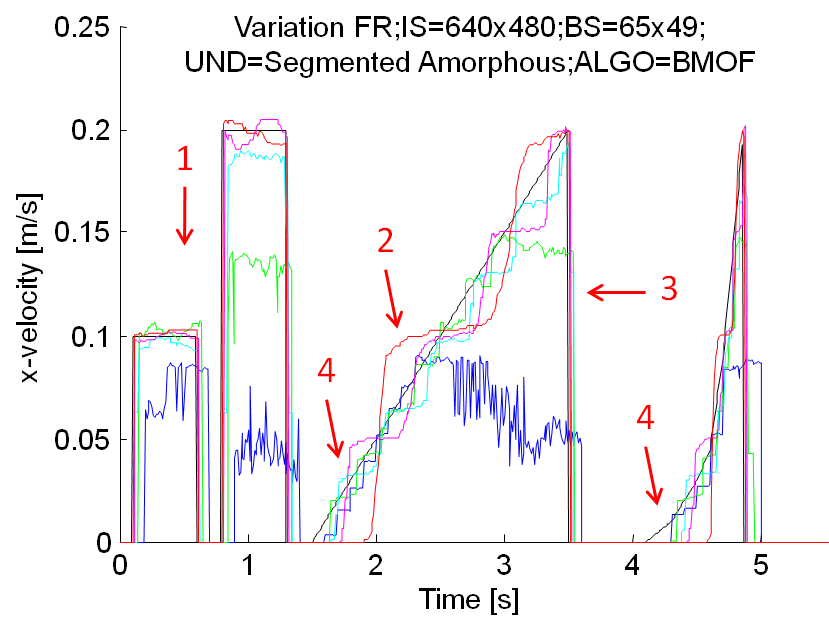
\includegraphics[width=0.50\textwidth]{graphic/Eval_IP_TS3_1_a.png}}\hfill
\subfigure[]{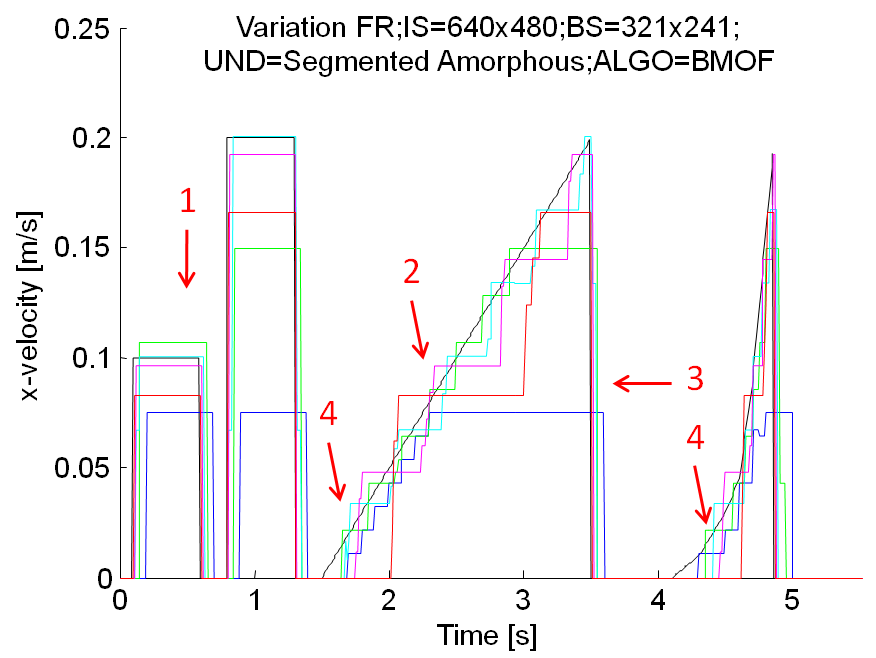
\includegraphics[width=0.50\textwidth]{graphic/Eval_IP_TS3_1_b.png}}
\subfigure[]{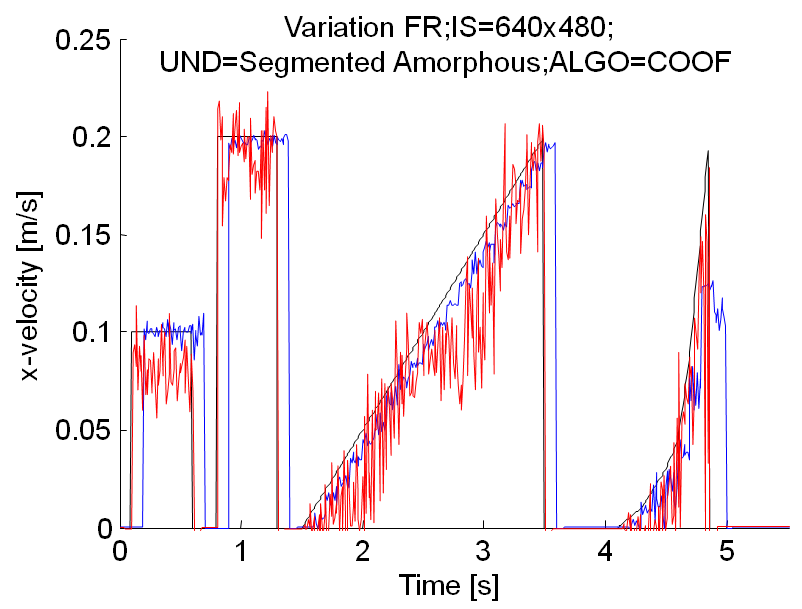
\includegraphics[width=0.50\textwidth]{graphic/Eval_IP_TS3_1_c.png}}
\subfigure[]{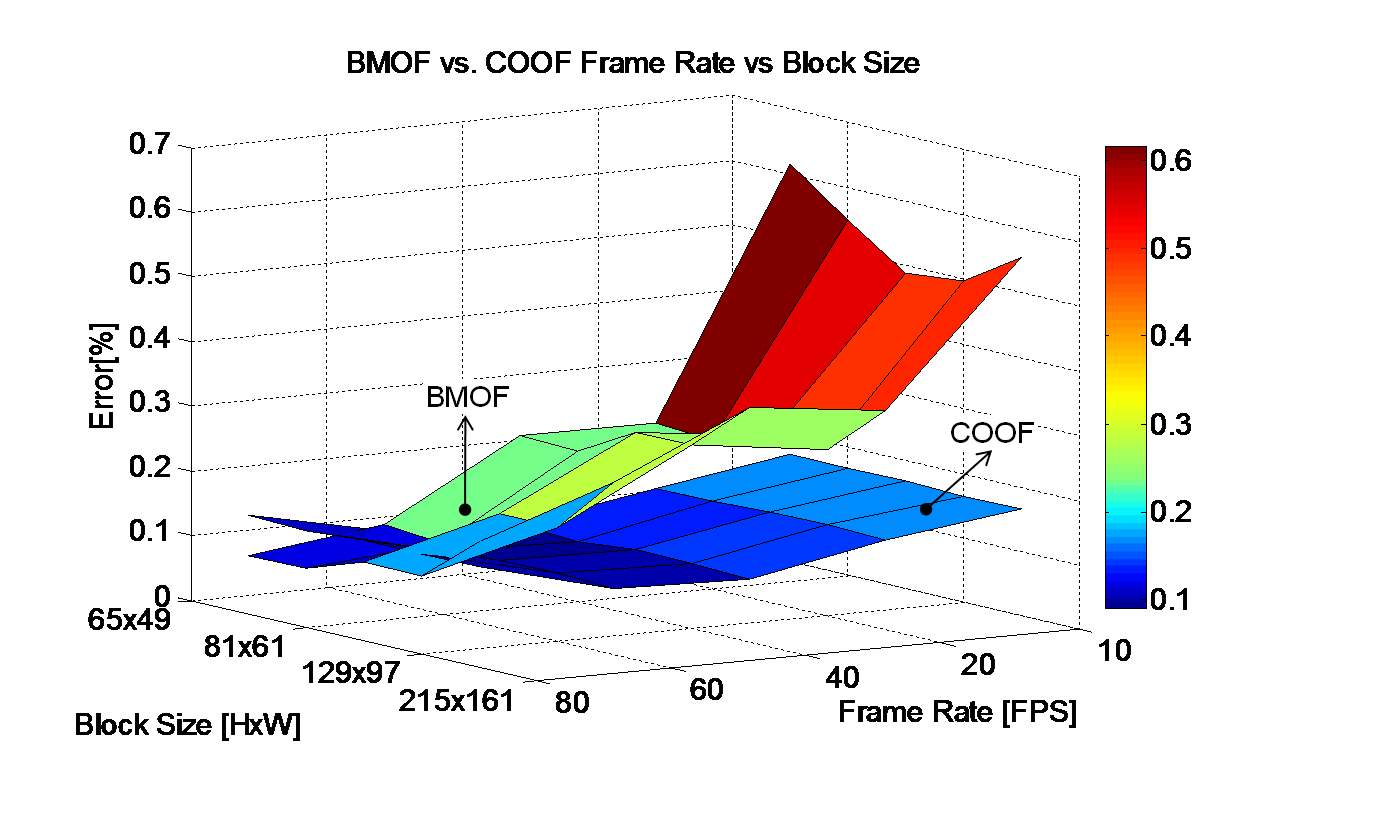
\includegraphics[width=0.50\textwidth]{graphic/Eval_IP_TS3_1_d.png}}
\begin{center}
\subfigure{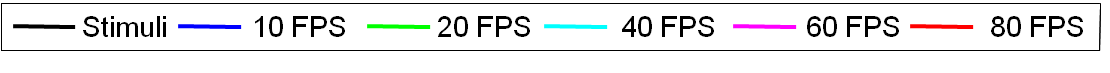
\includegraphics[width=1\textwidth]{graphic/Eval_IP_TS3_1_legend.png}}
\end{center}
\caption{Image Processing Result of Test Scenario 3: Translational analysis of BMOF and COOF} 
\label{fig:Eval_IP_TS3_1.png}
\end{figure}

The rotational behaviours of the two algorithms show many unexpected characteristics. By comparison to the coarse-grained block segmentation, the fine-grained segmentation of the \gls{BMOF} shows relatively satisfactory results. As we can see in diagramm \ref{fig:Eval_IP_TS3_2.png} (a), the highest frame rate provides the best results and the highest rotational speed detection. The lowest frame rate, as also presented in test scenario 1 (See \ref{fig:Eval_IP_TS1_3.png} (b), can not detect any movements satisfactorily and shows just a noisy signal. As expected, the \gls{COOF} algorithm also shows, in this scenario, a better rotational determination. On the other hand, it shows an unexpected behaviour related to the increase of the frame rate. As we can see in \ref{fig:Eval_IP_TS3_2.png} (c), the best results are captured with the highest frame rate. This result has almost no noise. With descending frame rate, the noise of the output signal is amplified, with the worst case visualised at the lowest frame rate. This effect could be based on the mentioned optical effects of the sample rate and the confusion of the tracked features, or could originate from an unexpected time variant limitation behaviour of the simulation.
Finally, a descriptive figure of the error characteristics of both algorithms is presented in \ref{fig:Eval_IP_TS3_2.png} (d). As we can see in the results of the \gls{COOF} surface, this algorithm improves the error characteristic with ascending frame rate. This is based on the fact that noise is reduced with ascending frame rate. In the result surface of the \gls{BMOF}, it can be seen that both variation values, frame rate and block size, have nearly equal influence on the error characteristic of the algorithm. This assumption is derived from the diagonally descenting surface of this algorithm.
 

\begin{figure}[H]
\subfigure[]{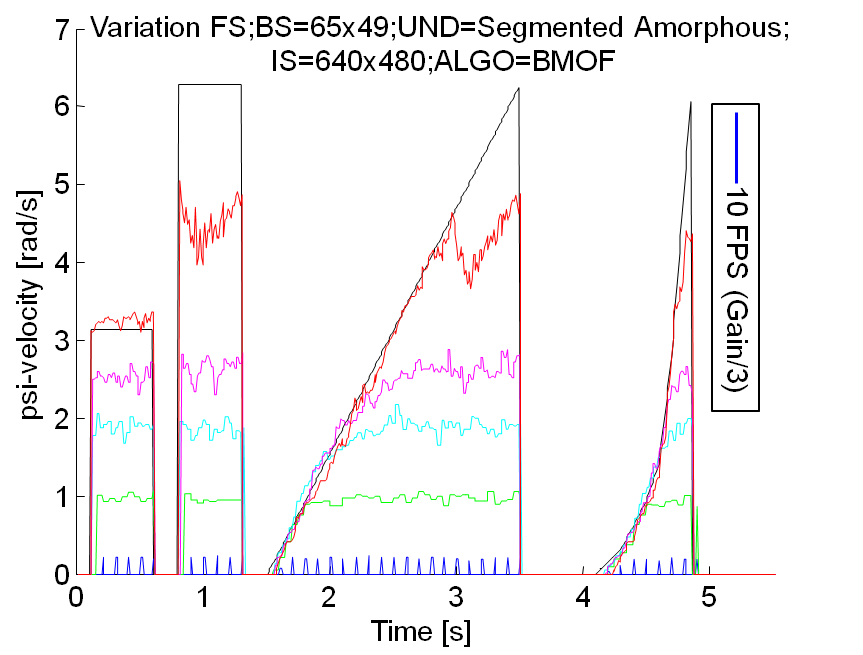
\includegraphics[width=0.50\textwidth]{graphic/Eval_IP_TS3_2_a.png}}\hfill
\subfigure[]{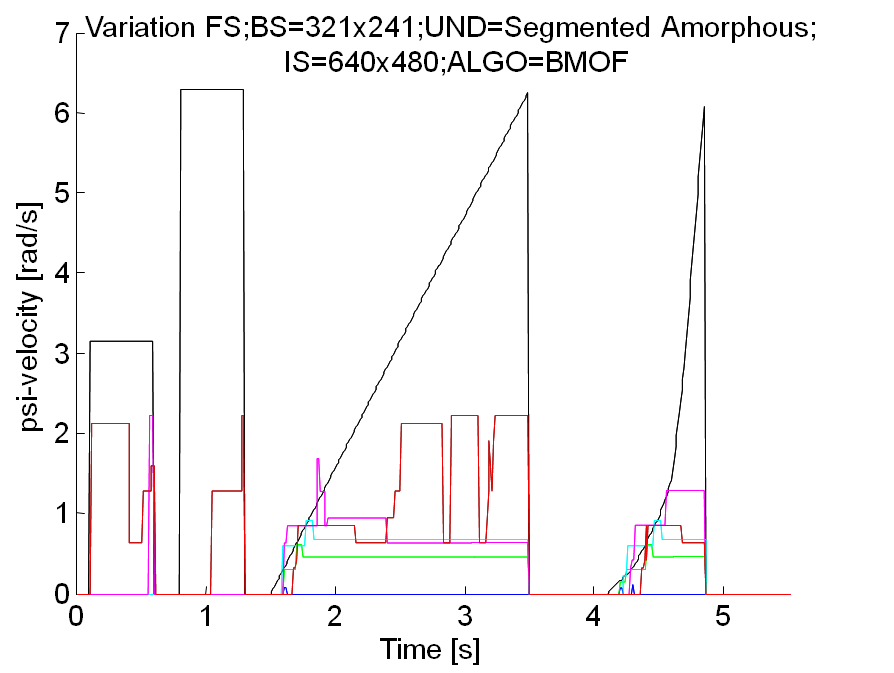
\includegraphics[width=0.50\textwidth]{graphic/Eval_IP_TS3_2_b.png}}
\subfigure[]{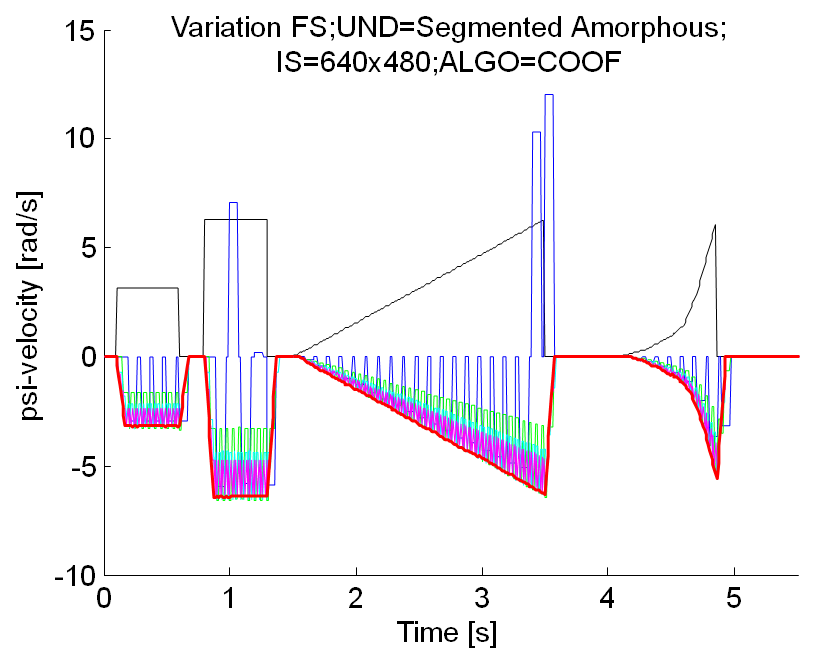
\includegraphics[width=0.50\textwidth]{graphic/Eval_IP_TS3_2_c.png}}
\subfigure[]{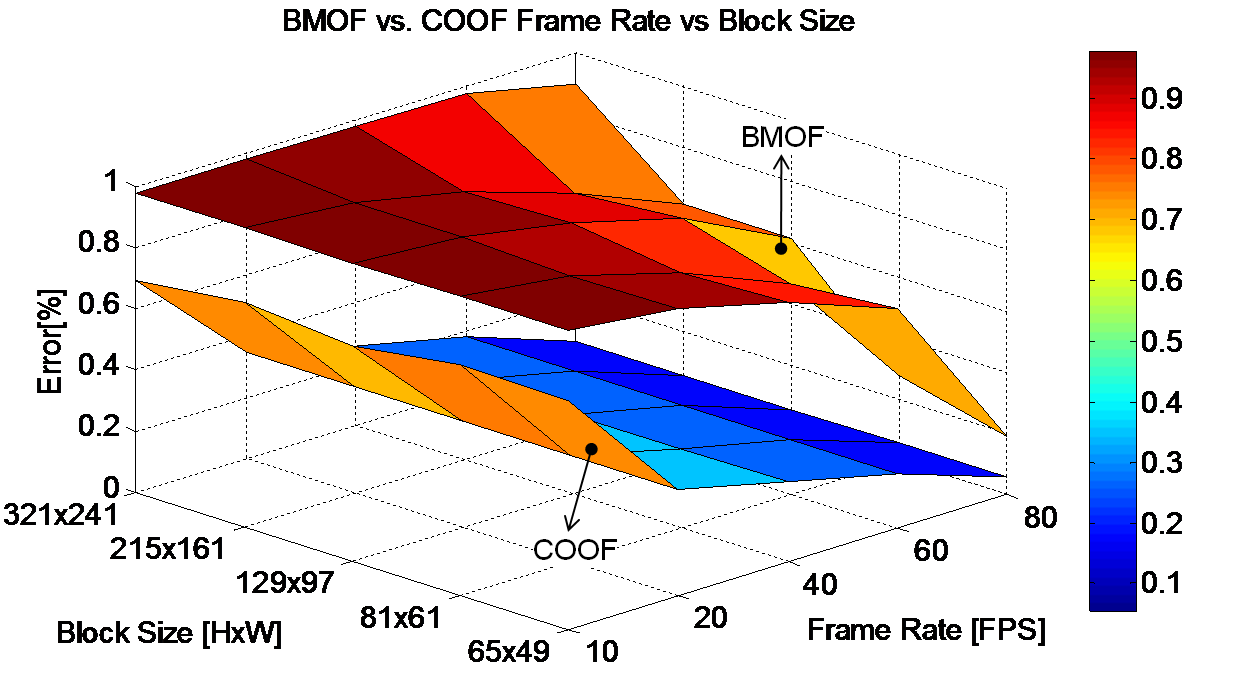
\includegraphics[width=0.50\textwidth]{graphic/Eval_IP_TS3_2_d.png}}
\begin{center}
\subfigure{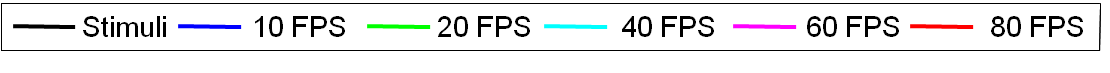
\includegraphics[width=1\textwidth]{graphic/Eval_IP_TS3_2_legend.png}}
\end{center}
\caption{Image Processing Result of Test Scenario 3: Rotational analysis of BMOF and COOF} 
\label{fig:Eval_IP_TS3_2.png}
\end{figure}

\subsubsection{Image Processing Test Scenario 4: Variation of Image Size reciprocal to the Sample Rate}
In this test scenario, the two parameters, image size and sample rate, are varied simultaneously. The aim thereby is to show the relation between the two parameters and the impact on the error amount of both algorithms \gls{BMOF} and \gls{COOF}. Additionally, it has to be analysed which parameter has the biggest influence on the error behaviour. The expected result of the comparison of the error characteristics of the two algorithms is that the \gls{COOF} algorithm will generally have a lower error surface in the analysis in rotational and translational behaviour, and will show a better best-case error-characteristic than the \gls{BMOF} algorithm. These assumptions base on the mentioned prospected characteristics, described in the previous test scenarios.

\subsubsection{Image Processing Results of Test Scenario 4}
A comparison of the focused algorithms, including the translational (a) and rotational (b) analysis, is shown in figure 
\ref{fig:Eval_IP_TS4_1.png}. Regarding the error rate of the translational behaviour of both algorithms, we can see that the expected error surface of the \gls{COOF} algorithm is truly lower than the error surface of the \gls{BMOF}. Also correctly expected in this case was the best case behaviour (\ref{fig:Eval_IP_TS4_1.png} (a) arrow No. 2) of the \gls{BMOF}. The pointed corner in the diagram shows that the best-case error value of the \gls{COOF} is lower than the corresponding best-case error-value of the \gls{BMOF} algorithm. An unexpected behaviour is that the error behaviours of both algorithms show an interesting response in the section of \ensuremath{40}\gls{FPS}. In this case, \gls{BMOF} shows a better error characteristic in comparison to the \gls{COOF} algorithm, which contains one of the biggest error values in this section.
The rotational behaviour, shown in \ref{fig:Eval_IP_TS4_1.png} (b), shows that both algorithms have the worst error characteristic in the section of the lowest sample rate. The \gls{BMOF} algorithm shows, especially in this section, an error of nearly 100\text{\%}. Furthermore, we can see that the \gls{BMOF} algorithm can only provide a satisfactory result between the sample rates of \ensuremath{60}\gls{FPS} and \ensuremath{80}\gls{FPS}. In contrast to that, the \gls{COOF} algorithm shows the first acceptable error behaviour at less than \ensuremath{20}\gls{FPS}. So the \gls{COOF} algorithm could be the correct one to realise a distributed error correction scheme with a sample rate of 20 \gls{FPS}.
Both diagrams show the relation to the two parameters, varied in this scenario. As we can see, the frame rate has a bigger impact to the error characteristic than the image size. This fact can be determined because the biggest variations of the output is shown in direction of the frame rate axis.

\begin{figure}[H]
\subfigure[]{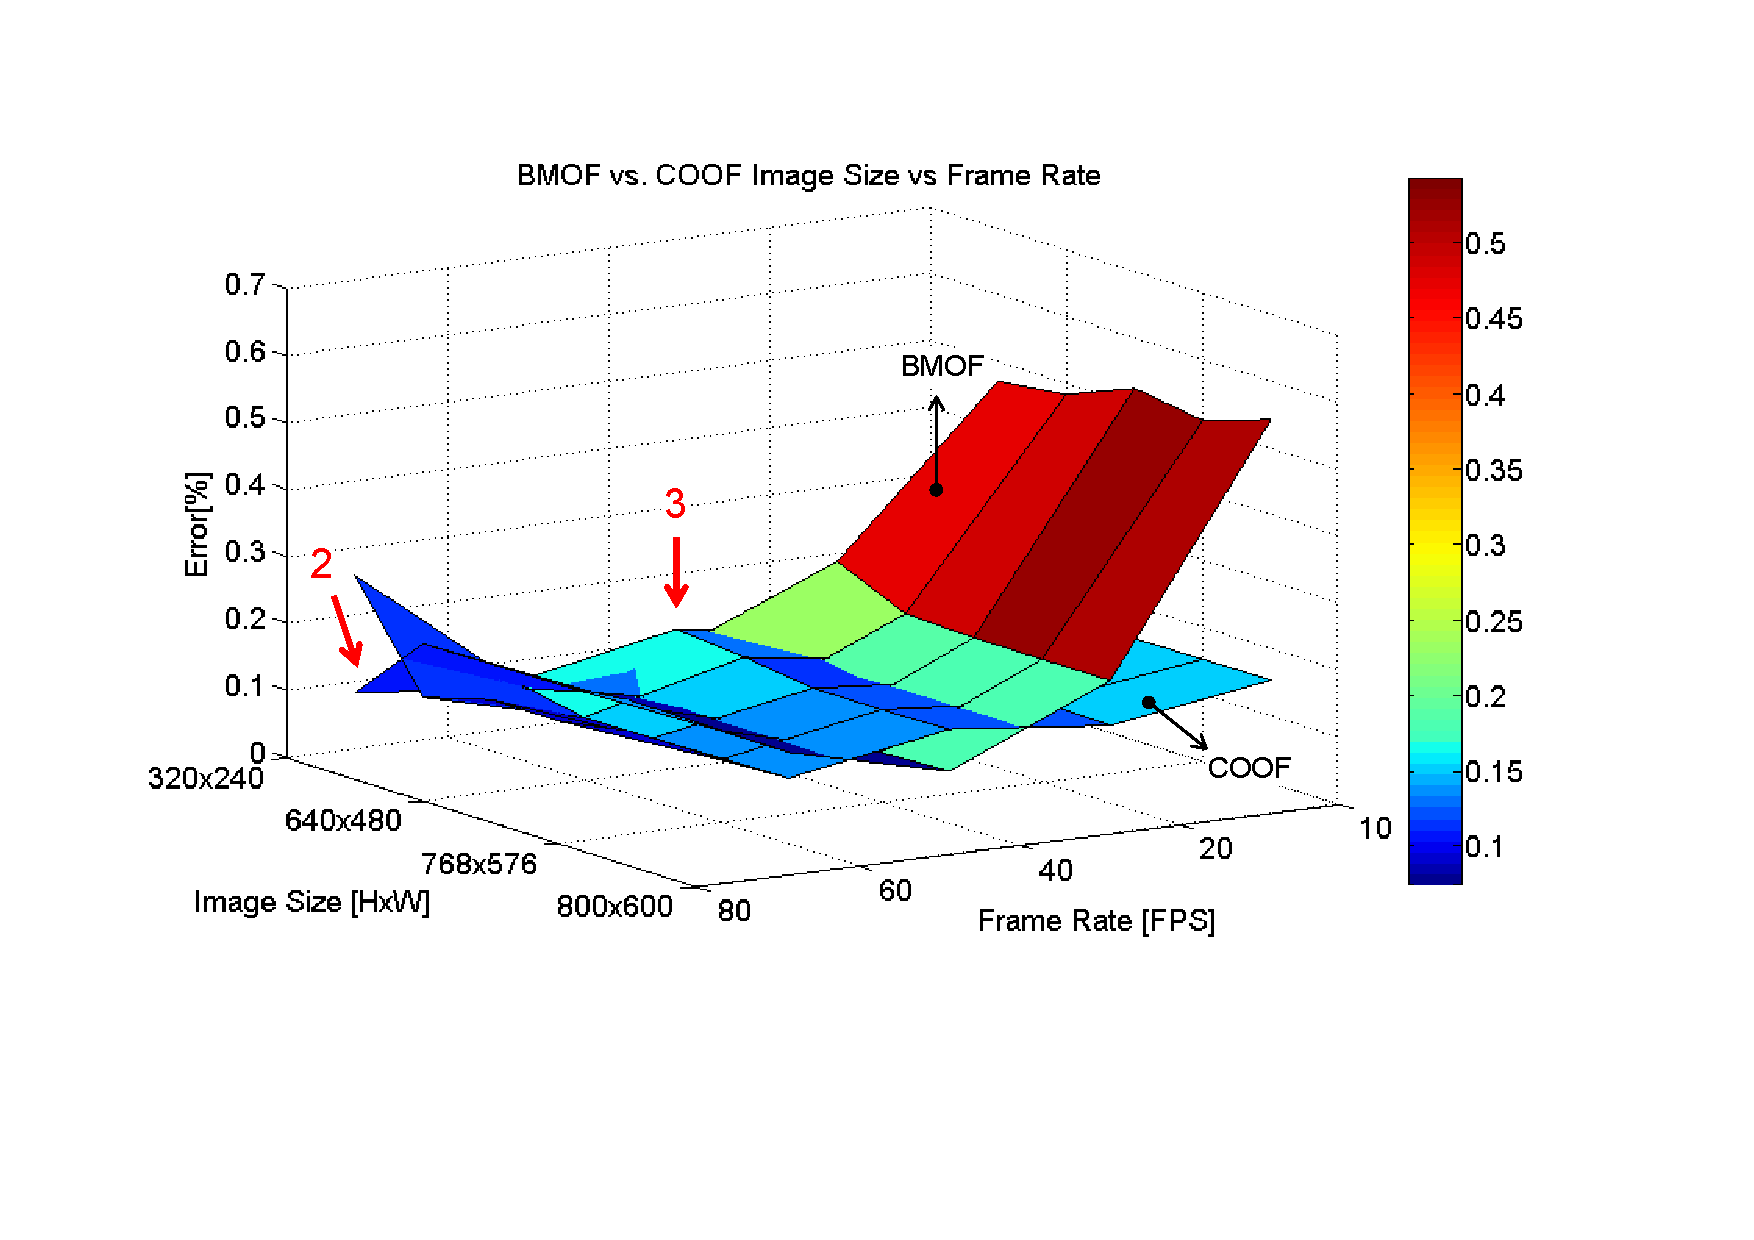
\includegraphics[width=0.50\textwidth]{graphic/Eval_IP_TS4_1_a.pdf}}\hfill
\subfigure[]{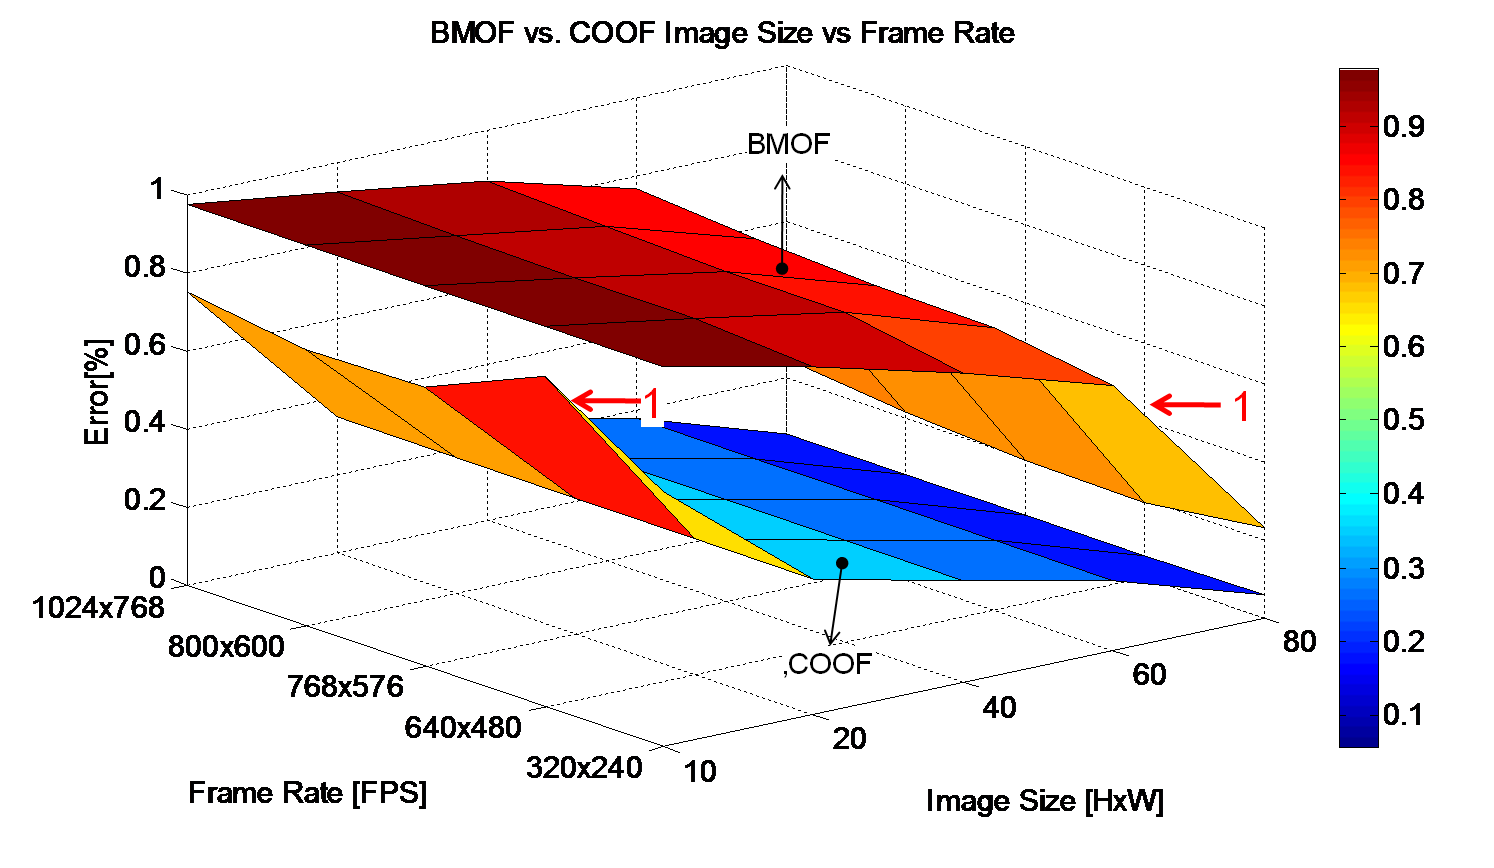
\includegraphics[width=0.50\textwidth]{graphic/Eval_IP_TS4_1_b.png}}
\caption{Image Processing Result of Test Scenario 4: Translational and Rotational analysis of BMOF and COOF} 
\label{fig:Eval_IP_TS4_1.png}
\end{figure}
%In this test scenario, the two parameters, image size and sample rate, are varied simultaneously. The aim thereby is to 
%Variation of Translation and Rotation Speed 
	%A:Variation of Underground
		 %Test Block Matching and COOF
		 %->Result The best config. of Block matching and COOF
	%B: Variation of Image size (Use config from A)
		%Test Block Matching and COOF
		  %Image Size is related with block size -> optimal config?
			%Image Size is not so much related to the funct. of COOF?(Expectation)
		%->Result of best and worst Image Size
	%Variation of frame Rate (Use Result from A and B)
		%Test Block Matching and COOF
		%->Result of best and worst frame Rate
%--------------------------------------------	


\subsection{Summary}
\label{mt:c:expResults:AnalysisofImageProcessing:Summary}
This chapter showed several interesting characteristics of the realised image processing simulations. Starting with the results of the first test case, it can be said that the error and precision characteristic was nearly the same for all tests. Some unexpected effects were found in these test cases which can be explained with the internal algorithm characteristics. Finally the variation of undergrounds shows that undergrounds with nearly the same contrast distribution have nearly the same results. Regarding the second test scenario, the variation of image sizes shows, unexpected an impact on the translational noise behaviour of the \gls{COOF} algorithm and the rotational speed limitation of the \gls{BMOF} algorithm. The translational behaviour of \gls{BMOF} and the rotational behaviour of \gls{COOF} show an insensitive attitude in relation to the image size variation. The variation of the frame rates shows a dramatically increasing impact of noise behaviour of the \gls{COOF} with increasing frame rate, and a limitation behaviour of maximum speed detection of the \gls{BMOF}. Furthermore, the results of the experiments of the frame rate variation show the unexpected behaviour of output signals' delay. Finally, the fourth test scenario demonstrated that the impact of the frame rate, in relation to the error of the output and input signal, is much higher than the error impact related to the image size.  

\section{Analysis of Control behaviour}
\label{mt:c:expResults:AnalysisofControlbehaviour}
This chapter focuses on the analysis of the body and position control behaviour. The aim thereby is to demonstrate the ideal control configuration for the final test analysis. So influences of the disturbances of the image processing are not regarded in this case. Therefore the analysis and optimisation of control is executed in this chapter with the sensor disturbances of the \gls{IMU} existing in reality only.
Regarding the mentioned theory of control systems in chapter \ref{mt:c:literature:s:Control_Systems_Characteristics}, the criteria of stability and performance measurement can be executed systematically in linear systems. Systems which include non-linearities can be linearised in one operating point of the non-linear component. In case of the quadrocopter plant, the set-point of the brushless controllers and the corresponding thrust are non-linear (See \ref{mt:c:DesignAndImplemetation:Sensors_and_Actuators}). So a strategy to fine tune the \gls{PID} controller parameters by regarding the non-linearity behaviour is presented in \ref{fig:AnalysisOfControlStrategy.pdf}
\footnote{This strategy was established in an interview with Prof. Dr. Kull and bases on the theory presented in \citebib{Kul10}}.
As we can see in the presented state chart, the first separation for further analysis steps is to determine if the plant is linear or not. In case of a linear plant, the methods presented in the figure and discussed in \ref{mt:c:literature:s:Control_Systems_Characteristics} can be executed. If the plant is non-linear, a linearisation at an operating point can be helpful to linearise the model and to execute the linear analysis systematically. In case of the quadrocopter, the linearisation at several operating points show the same unstable results 
(See \ref{fig:phi_psi_theta_lin_0} (a) and (b)). 

\begin{figure}[H]
\begin{center}
\subfigure[]{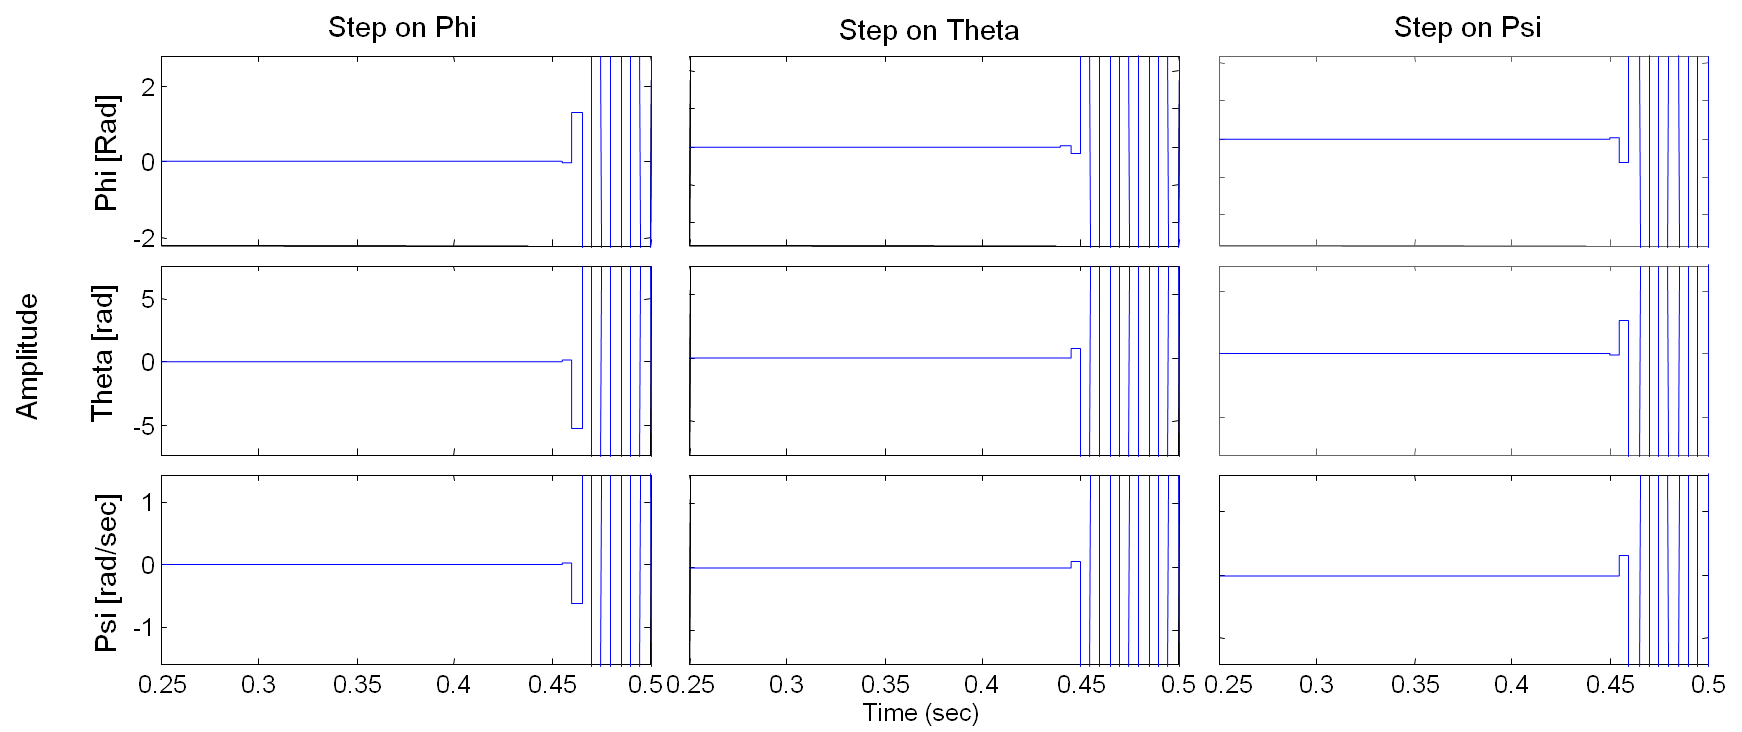
\includegraphics[width=1\textwidth]{graphic/phi_psi_theta_lin_0_step.png}}\hfill
\subfigure[]{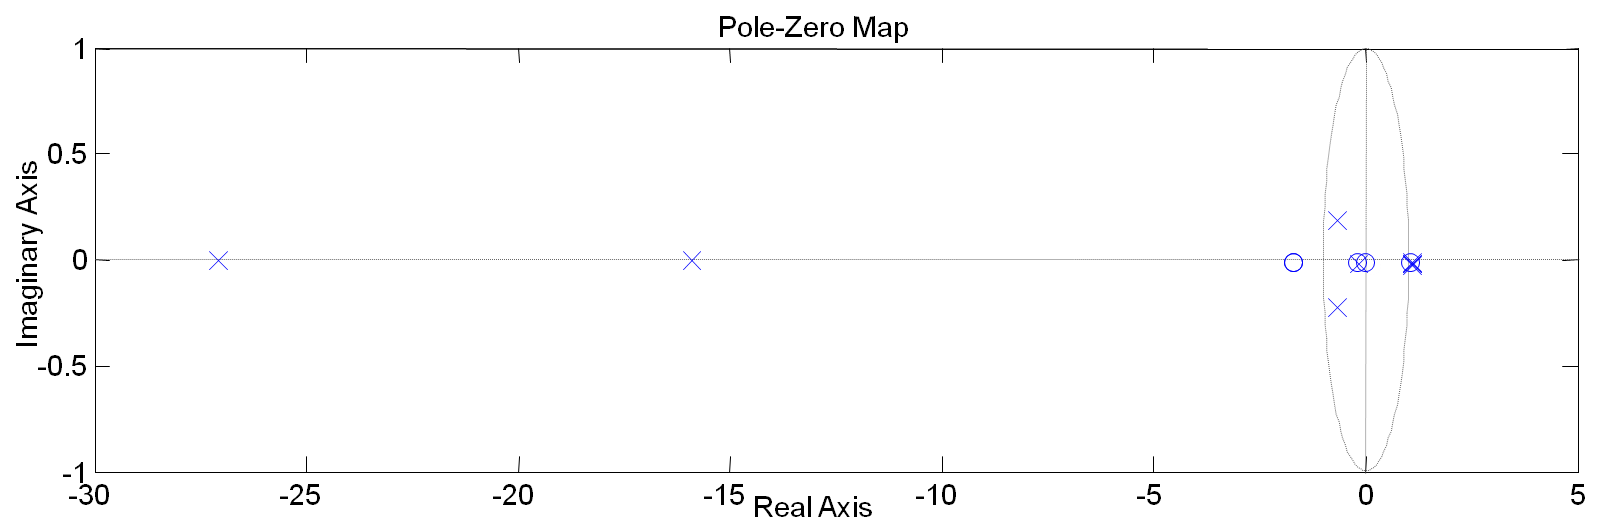
\includegraphics[width=1\textwidth]{graphic/phi_psi_theta_lin_0_pzmap.png}}
\caption{Step response and Pole-Zero map of linearised model} 
\label{fig:phi_psi_theta_lin_0}
\end{center}
\end{figure}

After the results of the linearised plant, the possibility to determine the optimal control parameters is the empirical method. 
This method presumes that the output values are independent from each other. In case of the quadrocopter model, the input values, which have an impact to the stability of the system, are the angles. These are independent from each other and do not need an uncoupling system. Such a system is a module integrated into the \gls{CLCS} that eliminates the influences of related output values. The further analysis and determination of the optimal \gls{PID} values for each controller was executed with the Simulink-Design-Optimization-toolbox \copyright \footnote{See \citebib{MatlabSDO11}}, which uses several optimisation and minimization algorithms to find the best suited configuration of the controller parameters.

\begin{figure}[H]
	\centering
		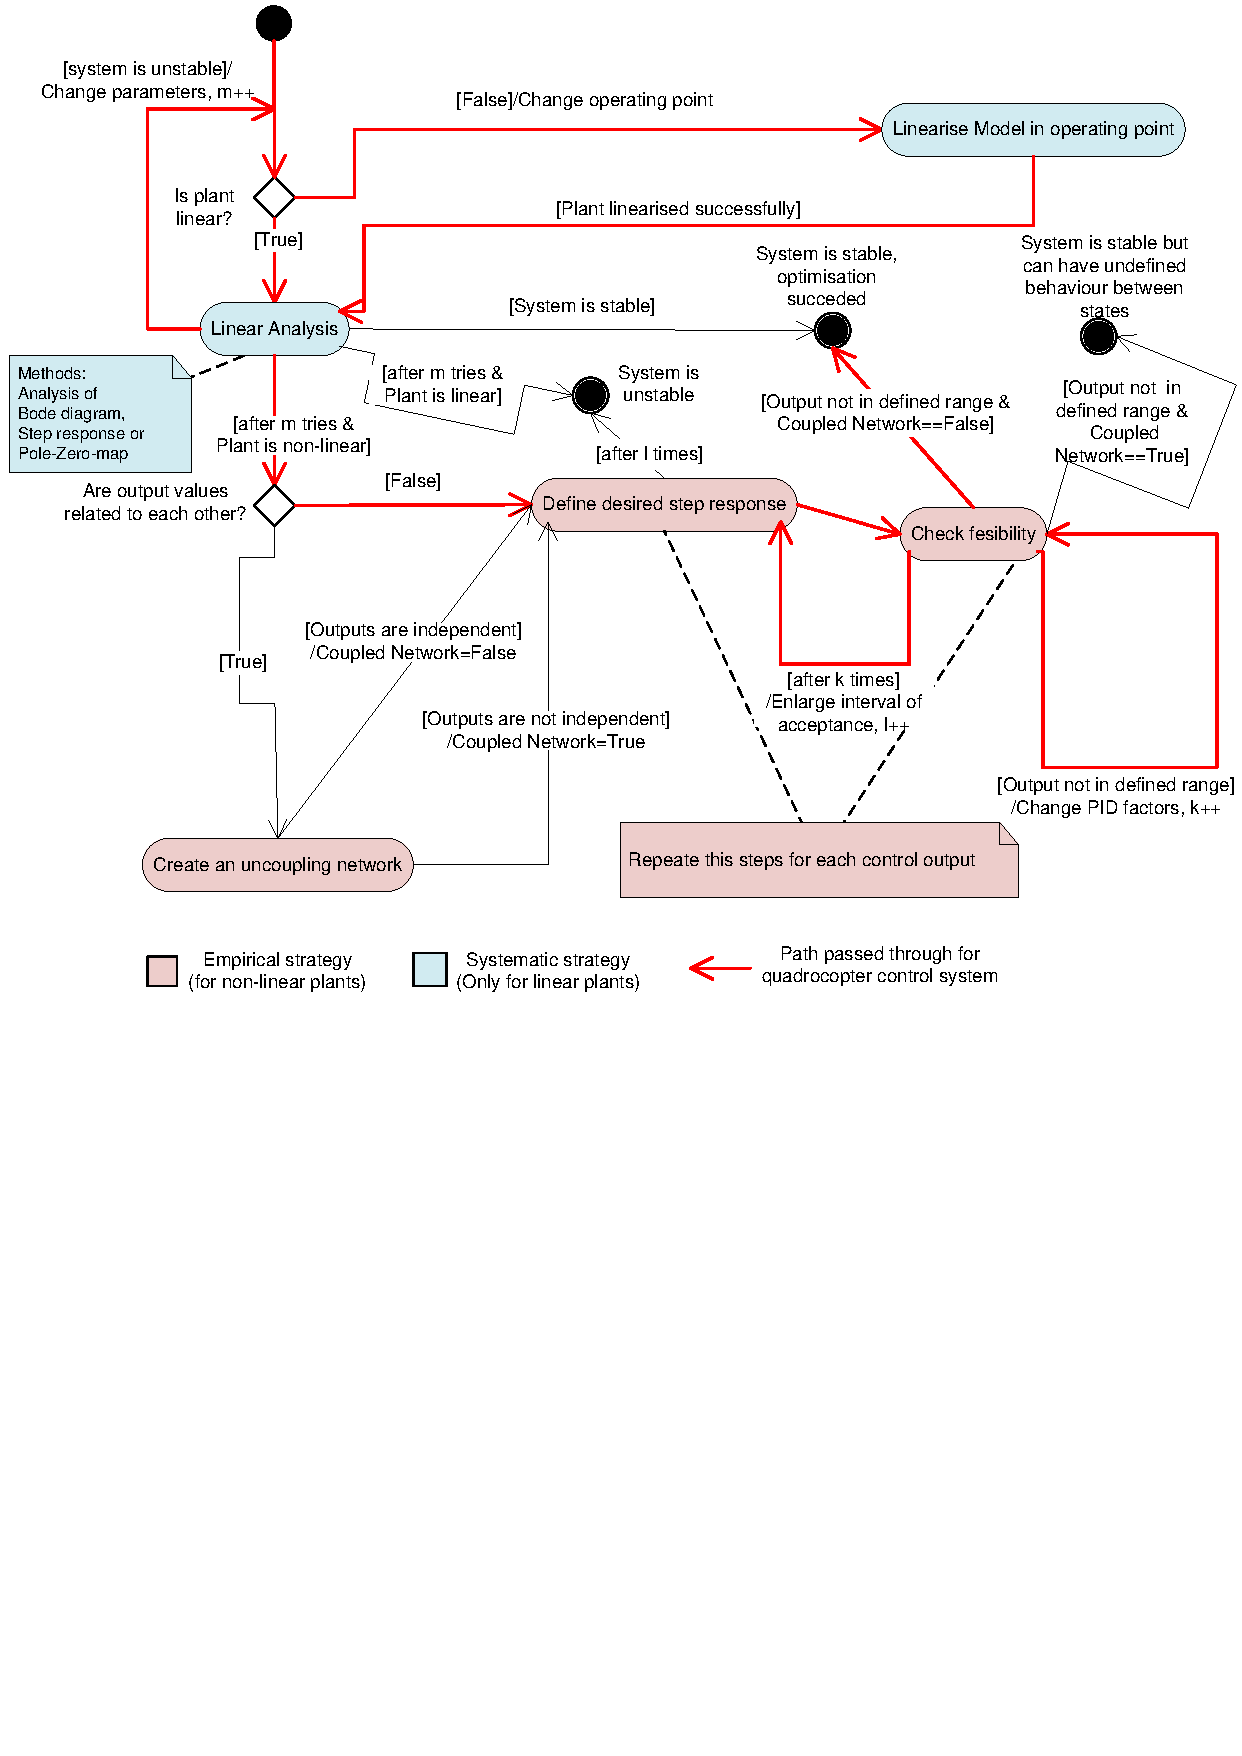
\includegraphics[width=1\textwidth]{graphic/AnalysisOfControlStrategy.pdf}
	\caption{Control tuning strategy for linear and non-linear CLCS}
	\label{fig:AnalysisOfControlStrategy.pdf}
\end{figure}

The following figure visualises the optimal tuned step response behaviour of the body \gls{PID} controllers. Thereby, the
optimisation algorithm shows two possible stable configurations, which differ in aspects of rise time, maximum overshoot 
and range of tolerance. The first stable configuration (\ref{fig:StepResponseBC_Phi_Theta_Psi} (a) and (b)) shows a stable behaviour until the step of 1.2 [rad] for body angles \ensuremath{\phi} and \ensuremath{\psi}. Compared with the second configuration 
(\ref{fig:StepResponseBC_Phi_Theta_Psi} (c) and (d)), which can only show a stable behaviour until the step value of 0.9 [rad], the first solution can be used to reach higher pitch and roll angles in flight. A possible drawback of the first configuration is the rise time, which is very high compared to the second configuration. 
A further cost of the high angle detection possibility is the oscillating behaviour of the first configuration. The second configuration thereby shows an increasing overshoot related to the increasing step stimulus.
Regarding the yaw behaviour of both configurations, we can see that the performance values are nearly the same, and show a very good rise time behaviour. The first configuration shows a high frequency oscillation behaviour. This could originate from the small motor invariances of the quadrocopter. An evidence for that could also be the fact that this behaviour also exists in the second configuration, but not with the same frequency. Finally, the second configuration will be used for further experiments and analysis because of the better steady state behaviour. These configurations' steady state behaviour will have a small influence to the optical position control performance. So this aspect is very important, and therefore the justification for this decision. Further, the second configuration can be improved with limiting the maximum angles of pitch and roll to 0.75 [rad]. This limitation guarantees an acceptable overshoot and prevents instabilities of the system. 

\begin{figure}[H]
\subfigure[]{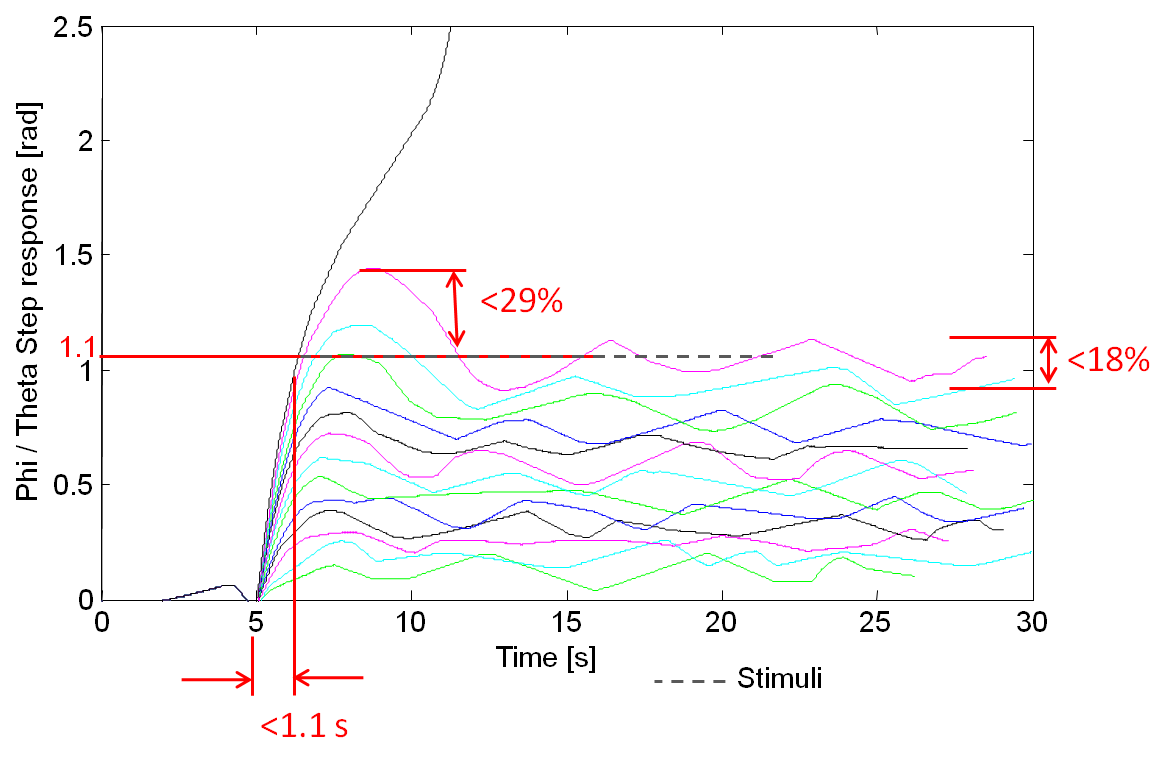
\includegraphics[width=0.50\textwidth]{graphic/StepResponseBC_Phi_Theta_Opt1.png}}\hfill
\subfigure[]{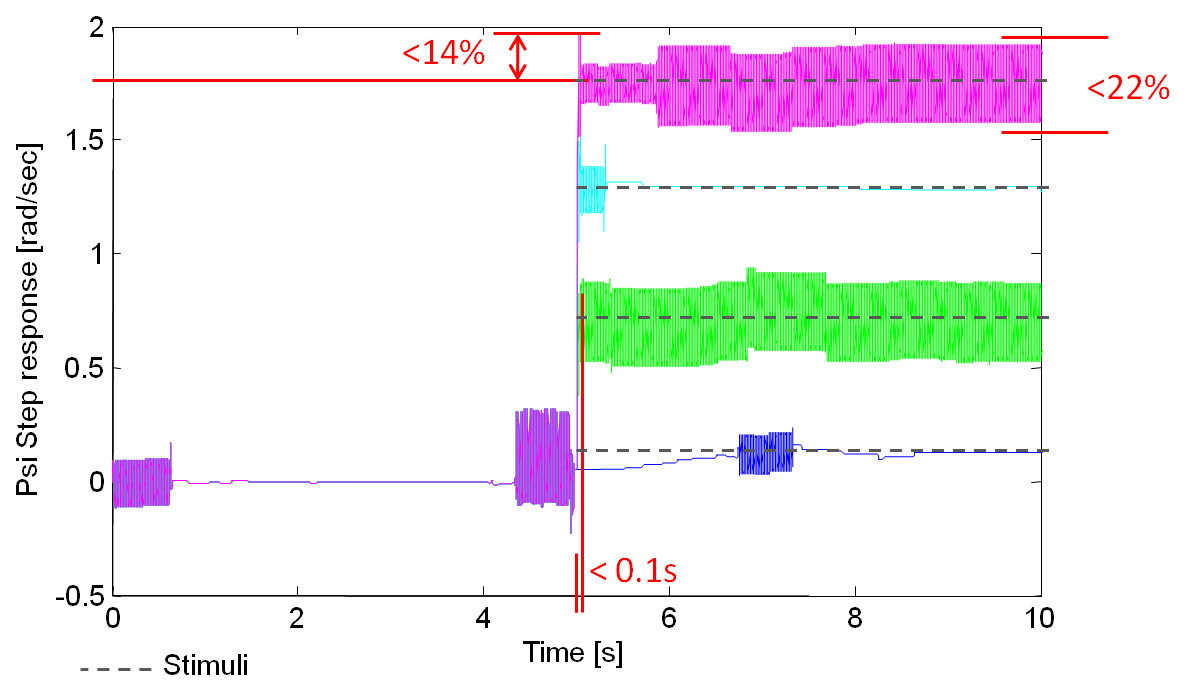
\includegraphics[width=0.50\textwidth]{graphic/StepResponseBC_Psi_Opt1.png}}
\subfigure[]{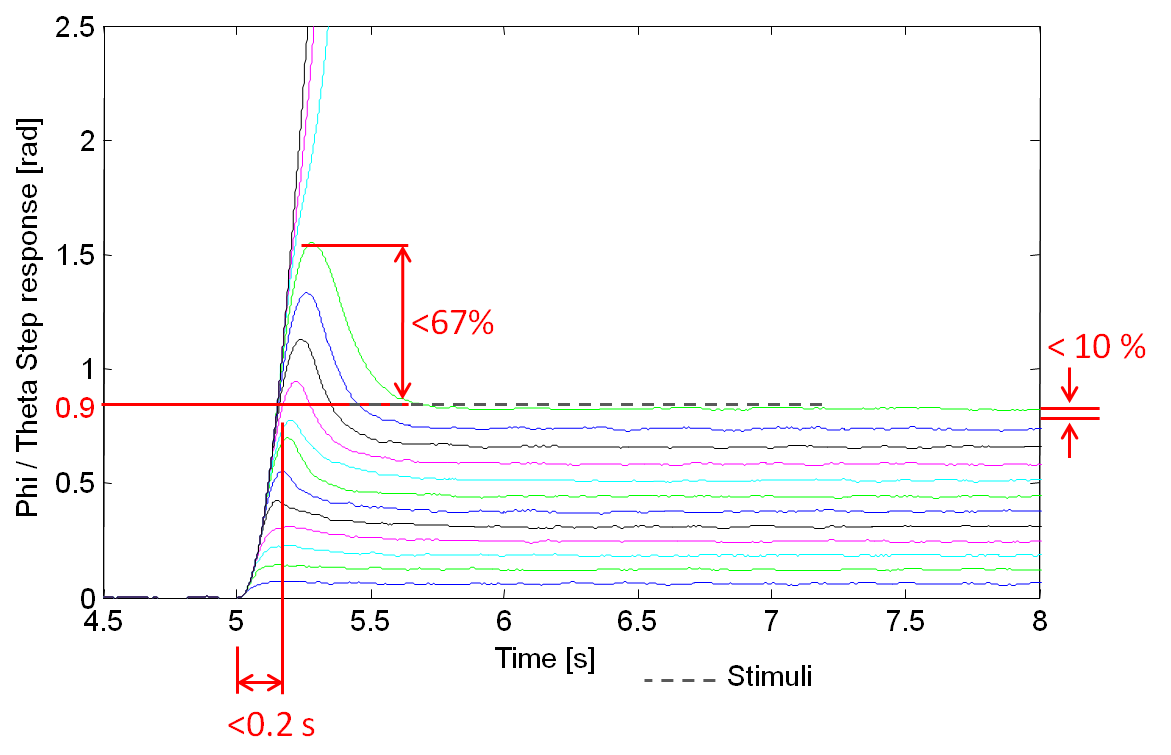
\includegraphics[width=0.50\textwidth]{graphic/StepResponseBC_Phi_Theta_Opt2.png}}
\subfigure[]{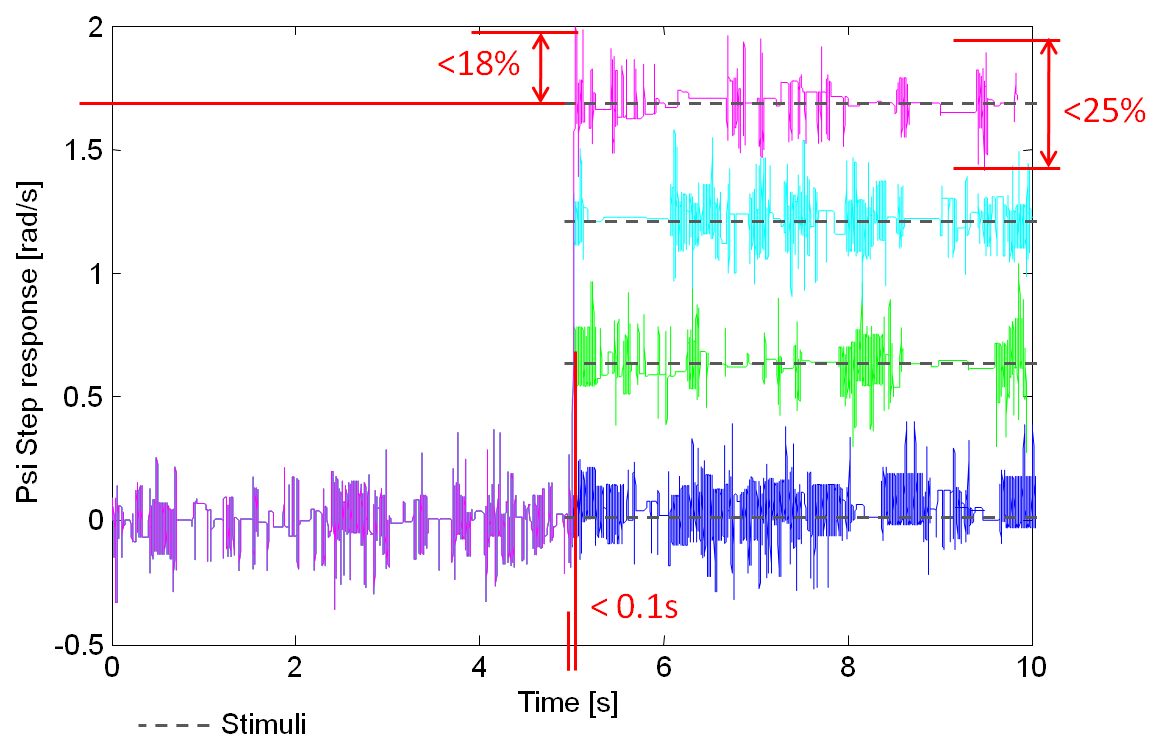
\includegraphics[width=0.50\textwidth]{graphic/StepResponseBC_Psi_Opt2.png}}
%\subfigure[]{\includegraphics[width=0.50\textwidth]{graphic/StepResponsePC_rPsi_Opt2.png}}
%\subfigure[]{\includegraphics[width=0.50\textwidth]{graphic/StepResponsePC_rPhi_Theta_Opt2.png}}
\caption{Results of Body PID Controller optimisation} 
\label{fig:StepResponseBC_Phi_Theta_Psi}
\end{figure}


The corresponding optimisation processing of the position \gls{PID} controllers is shown in \ref{fig:OptimisationPC_Phi_Theta_Psi}. 
Regarding the optimisation of the symmetrical axis angles \ensuremath{\phi} and \ensuremath{\theta}, we can see that the optimisation algorithms traverse some unstable configurations (See \ref{fig:OptimisationPC_Phi_Theta_Psi} (a)). Furthermore, several stable configurations were found by the optimiser, and the most suitable of these was chosen to realise the velocity position control for these axes. An interesting behaviour was found during the optimisation process of the optical \ensuremath{\psi} \gls{PID} controller. As visualised in diagram 
\ref{fig:OptimisationPC_Phi_Theta_Psi} (b)
the optimisation for psi was executed with a step disturbance. The aim of the controller is to equalise this movement  to zero as fast as possible. As we can see, the predicament of this optimisation is that the steady state error grows with the precision of the output signal. An example is demonstrated with the green (\ref{fig:OptimisationPC_Phi_Theta_Psi} (b) arrow No.1) and red 
(\ref{fig:OptimisationPC_Phi_Theta_Psi} (b) arrow No.2) regression lines, which show this behaviour. This phenomenon can be an important argument against an optical position correction of the \ensuremath{\psi} angle if the shown noise characteristic influences the position controller. Generally it can be assumed that the gyroscope sensor value and the corresponding control circle should work vastly better than the optical solution for this angle.
 
\begin{figure}[H]
\subfigure[]{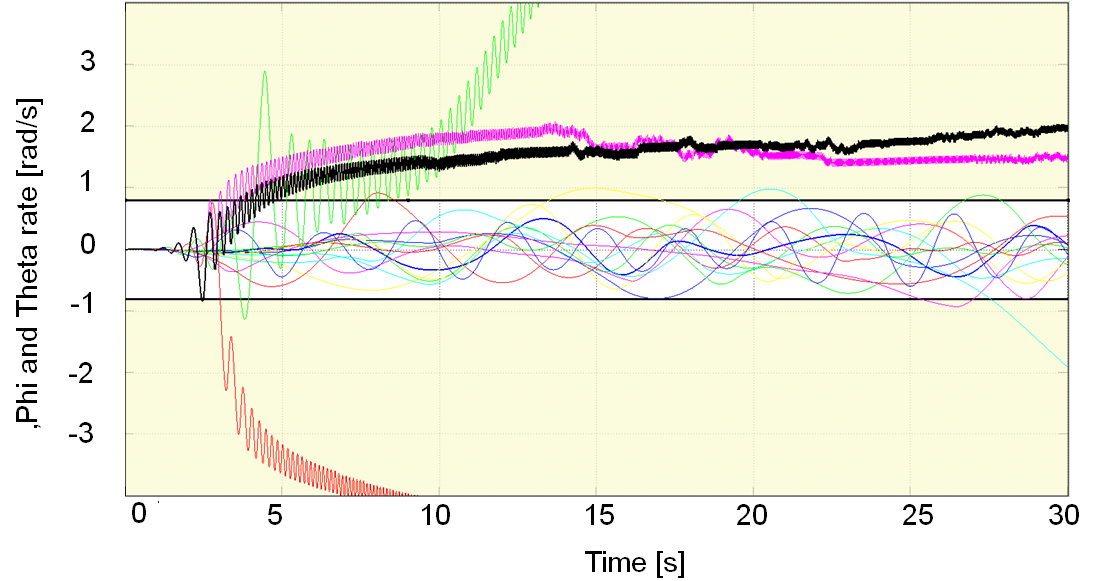
\includegraphics[width=0.50\textwidth]{graphic/PID_Optimisation_Opt_Phi_Theta.png}}\hfill
\subfigure[]{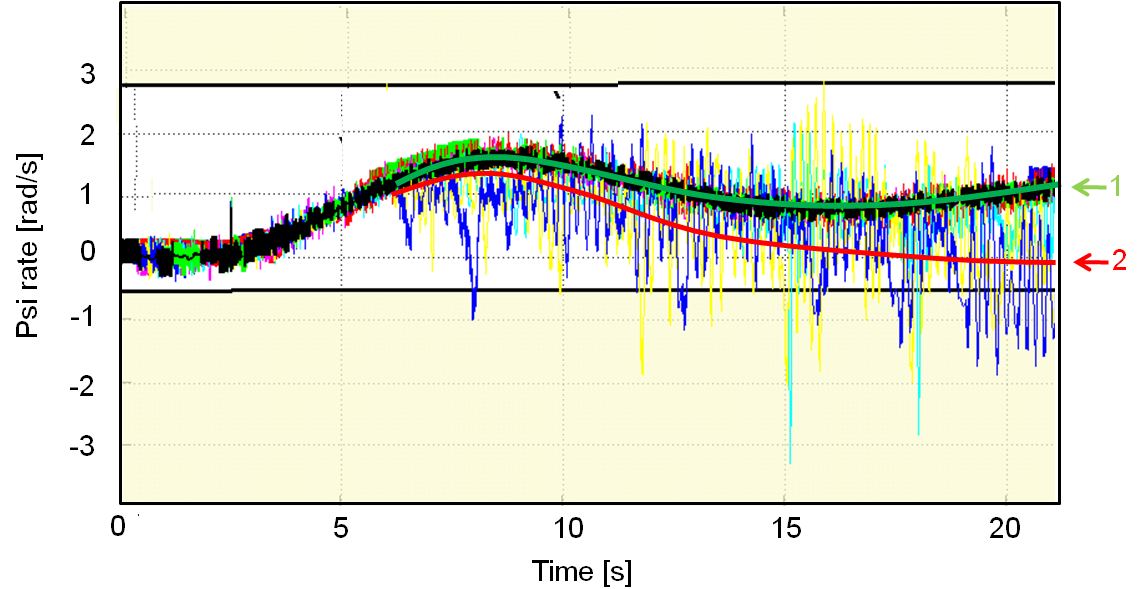
\includegraphics[width=0.50\textwidth]{graphic/PID_Optimisation_Opt_Psi.png}}
\caption{Results of Position PID Controller optimisation} 
\label{fig:OptimisationPC_Phi_Theta_Psi}
\end{figure}


\section{Analysis of Position Correction Scheme}
\label{mt:c:expResults:AnalysisofPositionCorrectionScheme}
This section focuses on the collaboration between optimised controller system and image processing. These consolidated components will be called 
"position correction scheme" within the scope of this project. Furthermore, the position correction scheme will be analysed under the execution of the following test scenarios presented in figure \ref{fig:PositionCorrectionSchemeTest.pdf} (a). As visualised, the test plan in this context is designed similar to the test plan of the image processing presented in \ref{fig:TestPlanOpticalFlow.png}. The difference here is that the test scenarios only focus on image size and frame rate variation, combined with a different model of 3D-trajectory stimulus. The decision in favour of these test scenarios is based on the results of the image processing analysis (See \ref{mt:c:expResults:AnalysisofImageProcessing} and 
\ref{mt:c:expResults:AnalysisofImageProcessing:Summary}). These results show that the biggest influence and the most interesting behaviour of the image processing originates from the variation of frame rate and image size. Additionally, the stimulus is classified here in three segments. All test scenarios executed with the rotational and translational configuration, presented in 
\ref{fig:PositionCorrectionSchemeTest.pdf} (b), and with an uplift stimulus that elevates the quadrocopter to a hovering state. For visualisation reasons, the rotational test is executed as a mixture of a translational and rotational part. Otherwise the 3D-Trajectory would be just a point, and so unsuitable for demonstration. The goal of these test stimuli is to show how the position correction scheme reacts under different conditions. Another aspect of segmentation is the different performance of regarded algorithms in case of rotation, translation and hovering tests.

\begin{figure}[H]
\subfigure[]{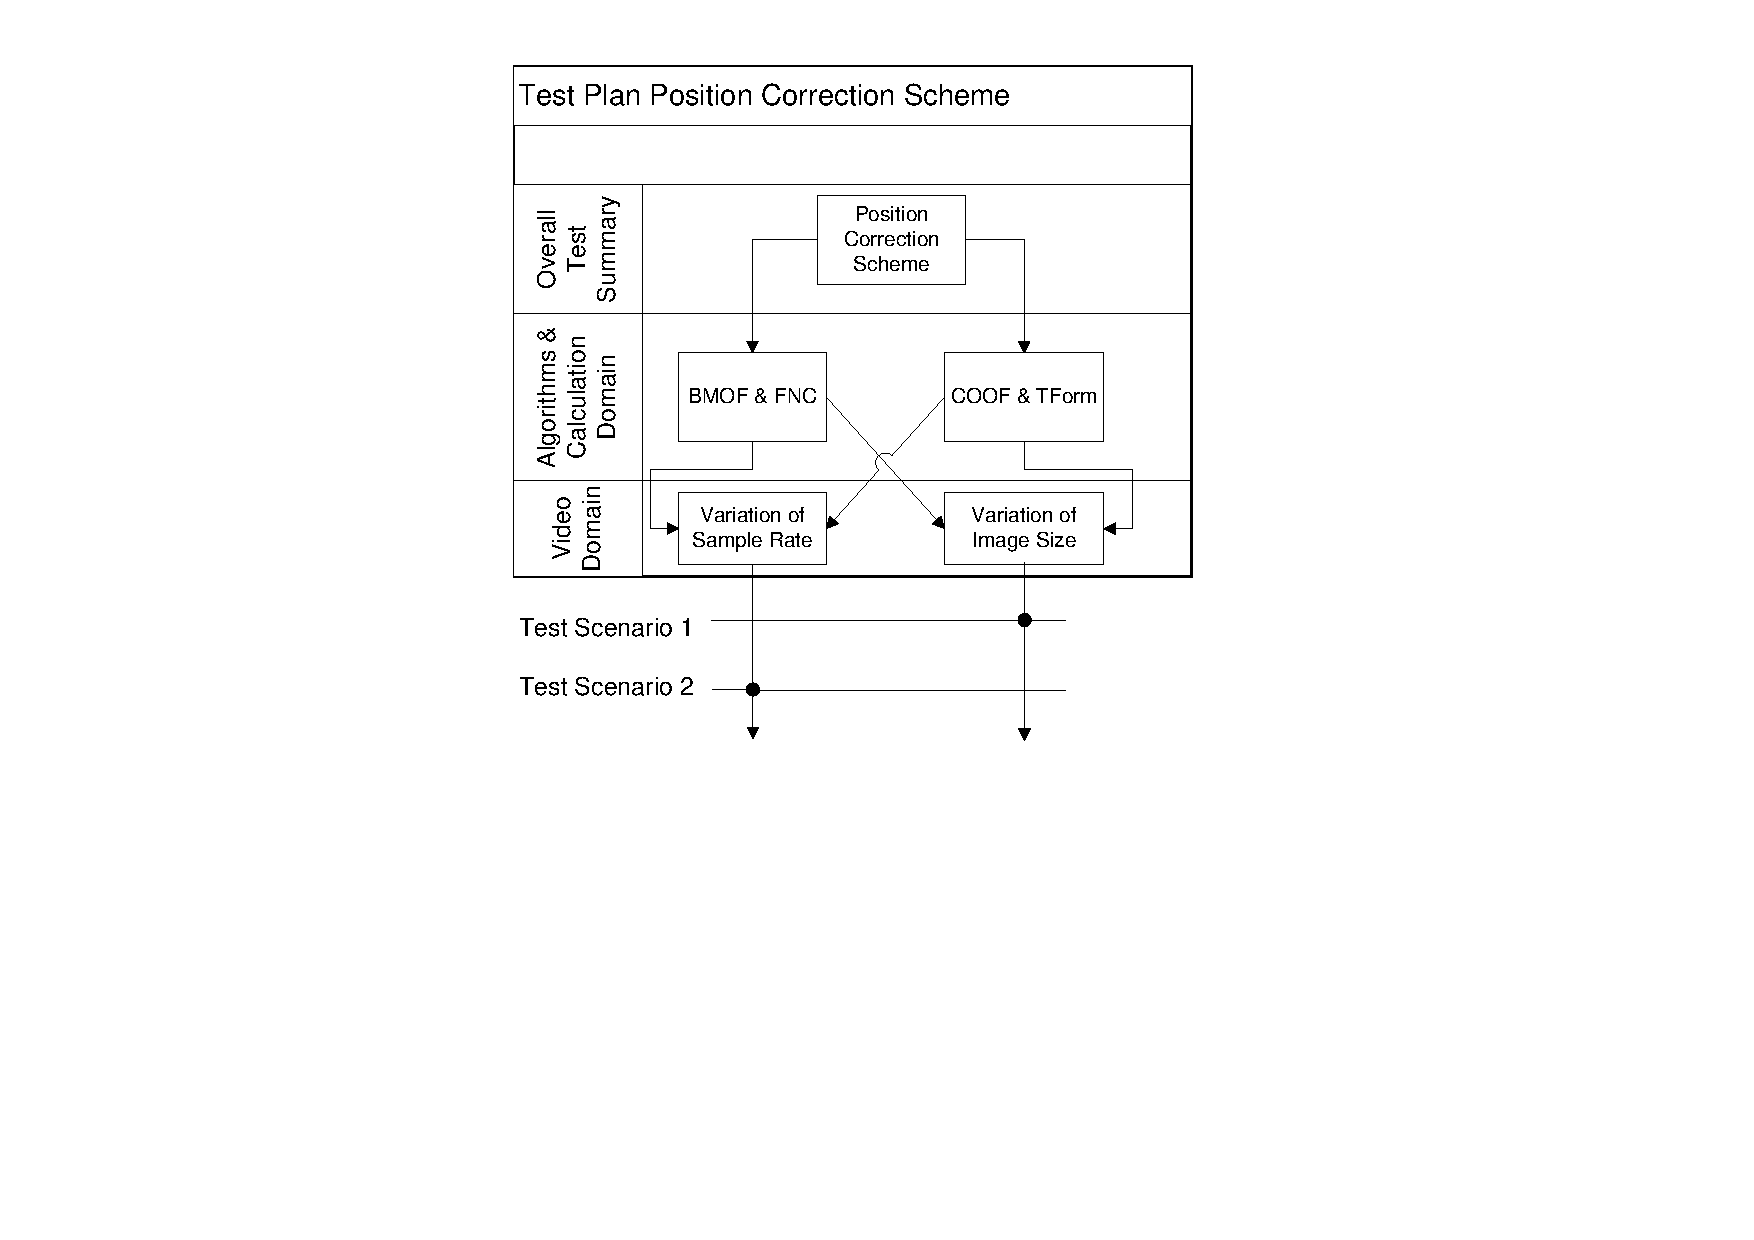
\includegraphics[width=0.50\textwidth]{graphic/TestPlanPositionCorrectionScheme.pdf}}\hfill
\subfigure[]{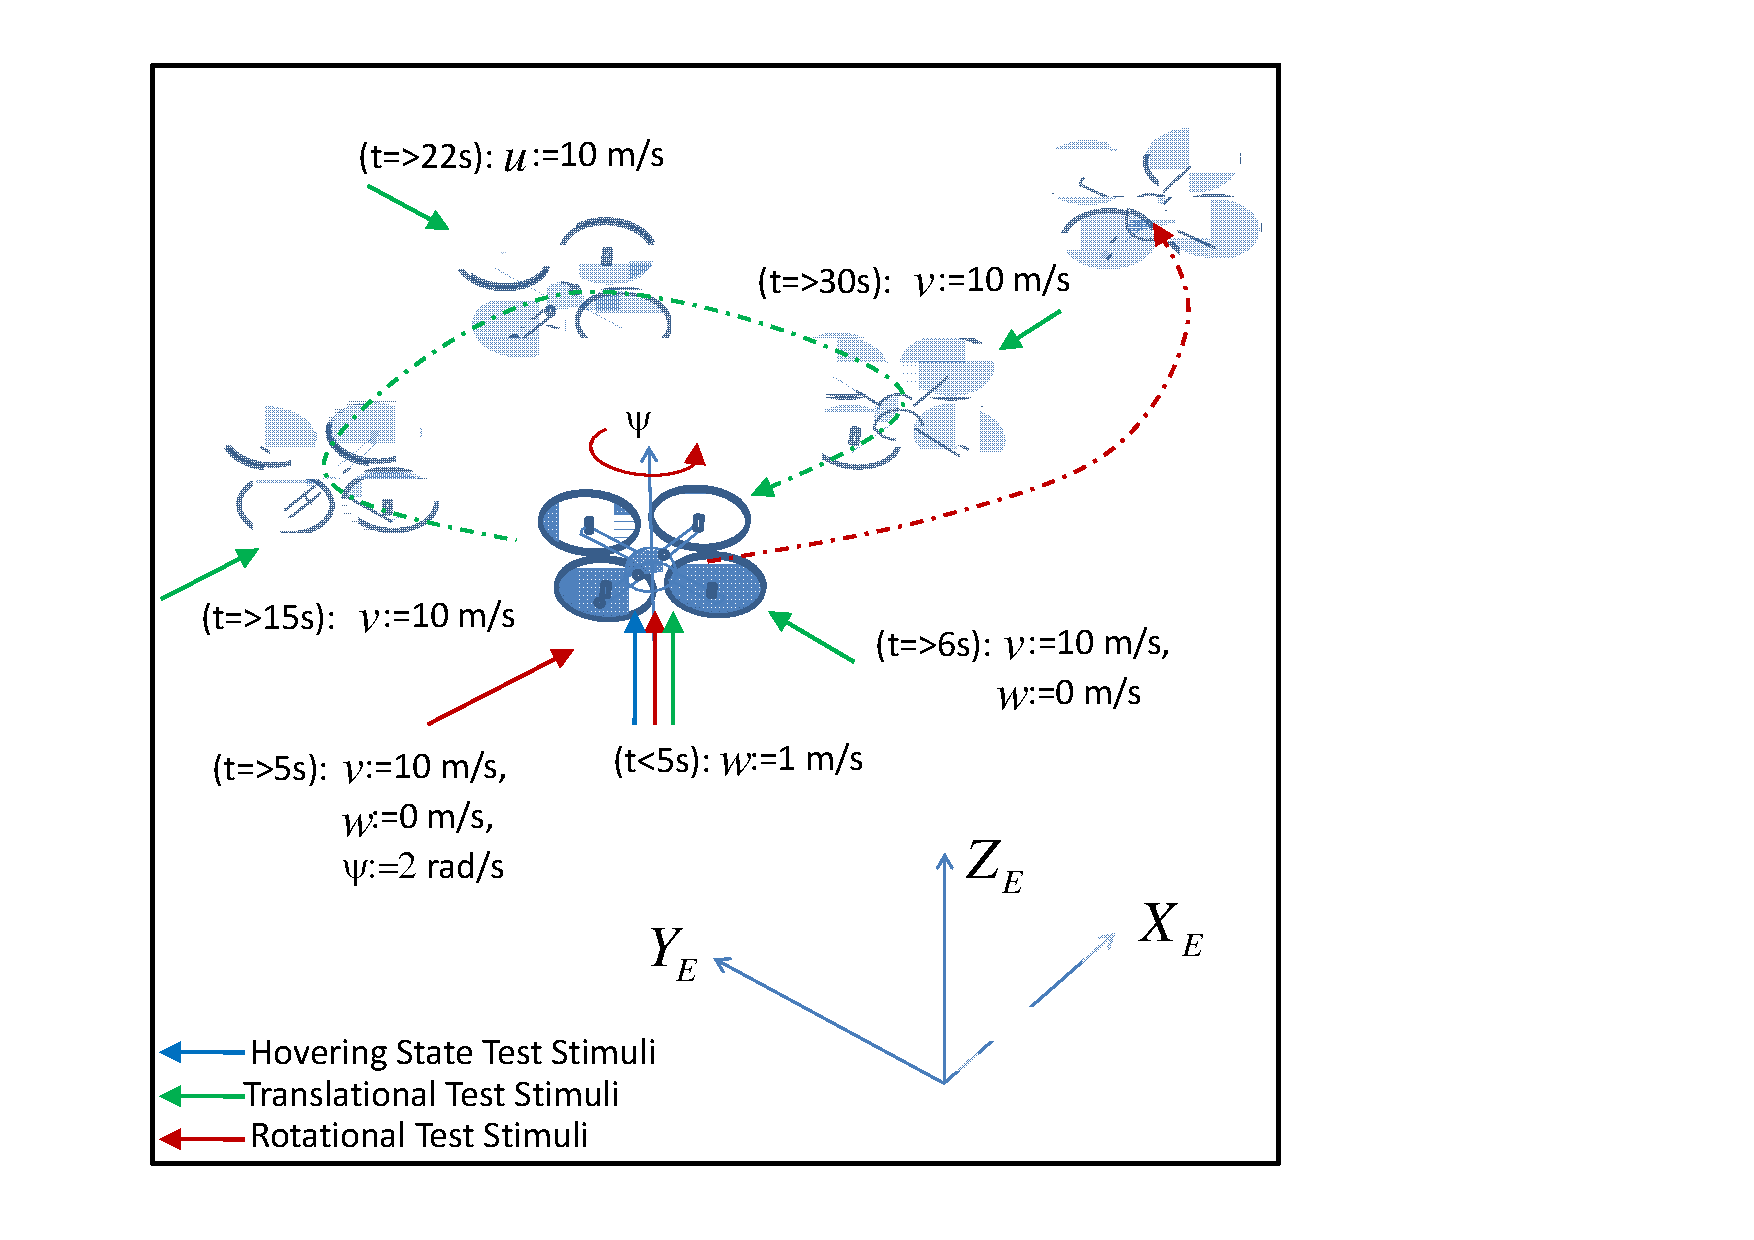
\includegraphics[width=0.50\textwidth]{graphic/PositionCorrectionSchemeTest.pdf}}
\caption{Test facility for hovering, rotational and translational position correction tests} 
\label{fig:PositionCorrectionSchemeTest.pdf}
\end{figure}


\subsection{Test Scenarios, Expectations and Results}

\subsubsection{Position Correction Scheme Test Scenario 1: Variation of Sample Rate}
One of the aims of this test scenario is to show the influence of the sample rate in relation to the introduced testing facility. To achieve this, the mentioned stimuli are executed with the introduced sample rates of 
10, 20, 40, 60, 80 FPS, introduced in chapter \ref{mt:c:expResults:AnalysisofImageProcessing}. The expected quality of the position correction scheme will be strongly related to the results presented in 
\ref{mt:c:expResults:AnalysisofImageProcessing:Summary}. As mentioned, the variation of frame rate show a big impact to the noise behaviour of the \gls{COOF} and the limitation behaviour of the \gls{BMOF} algorithm. Furthermore, signals of both algorithms show a delay characteristic, especially in the area of low sample rates. So these algorithms will show their mentioned strengths and weaknesses in the following 3D-Trajectories.

\subsubsection{Position Correction Scheme Results of Test Scenario 1}

As expected, the impact of the maximum speed limitation of the \gls{BMOF} algorithm is enormous. As we can see in figure 
\ref{fig:PCS_TS1_BMOF_COOF_Trans.pdf} (a), the 3D-Trajectories are deformed with decreasing sample rate to the direction of the \ensuremath{X_E} and \ensuremath{Y_E} axis. So this test shows, in a very suitable example, how the speed limitation of an image processing algorithm can influence the position correction scheme (See corresponding 2D-Trajectory in \ref{fig:Eval_IP_TS3_1.png} (a)). In contrast to the speed limited \gls{BMOF} algorithm, the \gls{COOF} algorithms' 3D-Trajectories are very precise (See \ref{fig:PCS_TS1_BMOF_COOF_Trans.pdf} (b)). Also correctly expected was the disturbance of the noise behaviour of this algorithm. As visualised in figure \ref{fig:PCS_TS1_BMOF_COOF_Trans.pdf} (b), the best results are not executed at the highest sample rate, but with a sample rate of middle image sizes. So it is demonstrated that the 
\gls{COOF} algorithm shows the most suitable results with an average signal delay, and also an average noise behaviour, in the translational position correction tests.

\begin{figure}[H]
\subfigure[]{\includegraphics[width=0.50\textwidth]{graphic/PCS_TS1_BMOF_Trans.png}}\hfill
\subfigure[]{\includegraphics[width=0.50\textwidth]{graphic/PCS_TS1_COOF_Trans.png}}
\begin{center}
\subfigure{\includegraphics[width=1\textwidth]{graphic/PCS_TS1_Legend.png}}
\end{center}
\caption{Position Correction Scheme Results of Test Scenario 1: Translational Test 3D-Trajectory of BMOF and COOF}
\label{fig:PCS_TS1_BMOF_COOF_Trans.pdf}
\end{figure}

The rotational tests of this scenario show some interesting characteristics. Starting with the \gls{BMOF} algorithm, we can see an unstable behaviour which is visualised as diverging spiral that climbs in higher and higher orbits. This instability is based on the unsuitable image processing rotational performance of the \gls{BMOF} algorithm at the lowest sample rate (See \ref{fig:Eval_IP_TS3_1.png}(a)). The further sample rates show a suitable result and visualise the S-form curve which is executed by the control system to stabilise the yaw-rotation and  
is coincident with the translational drift. Opposed to the characteristics of the \gls{COOF} translational behaviour, the rotational 3D-Trajectories of this algorithm show a stable but different from expected behaviour. The best-suited configuration in this case is the highest sample rate, because it shows the shortest 3D-Trajectory. But compared to the other 3D-Trajectories, the difference is not as big as the impact of a 80 \gls{FPS} sample rate in relation to the transmission or the image processing costs of the complete system.   

\begin{figure}[H]
\subfigure[]{\includegraphics[width=0.50\textwidth]{graphic/PCS_TS1_BMOF_Rot.png}}\hfill
\subfigure[]{\includegraphics[width=0.50\textwidth]{graphic/PCS_TS1_COOF_Rot.png}}
\begin{center}
\subfigure{\includegraphics[width=1\textwidth]{graphic/PCS_TS1_Legend.png}}
\end{center}
\caption{Position Correction Scheme Results of Test Scenario 1: Rotational Test 3D-Trajectory of BMOF and COOF}
\label{fig:PCS_TS1_BMOF_COOF_Rot.pdf}
\end{figure}

The next graphics visualise the hovering state behaviour of both algorithms for a time period of 60 seconds.
Starting with the \gls{BMOF} algorithm, visualised in \ref{fig:PCS_TS1_BMOF_COOF_Hov.pdf} (a) and (b), we can see the same unsatisfactory behaviour for a sample rate of 10 \gls{FPS} as demonstrated in the translational tests. As obviously visualised in 
\ref{fig:PCS_TS1_BMOF_COOF_Hov.pdf} (b), the blue 3D-Trajectory hovers over a concrete closed area, but drifts arbitrary.
Beside this, all other hovering tests are satisfactory, even the hovering state with 20 \gls{FPS}. Regarding the hovering state behaviour of the \gls{COOF} algorithm, we can see that the frame rate of 10 \gls{FPS} shows a better result, due to the smaller area of hovering, than the maximum frame rate of 80 \gls{FPS} (See \ref{fig:PCS_TS1_BMOF_COOF_Hov.pdf} (d)). This characteristic is also visualised in graphic 
\ref{fig:PCS_TS1_BMOF_COOF_Hov.pdf} (c), and could be the expected impact of noise which increases with increasing frame rate in context of the \gls{COOF} algorithm. Furthermore, this noise behaviour of the \gls{COOF} algorithm is also related to the image size and will be focused on in the second test scenario.

\begin{figure}[H]
\subfigure[]{\includegraphics[width=0.50\textwidth]{graphic/PCS_TS1_BMOF_Hov_All.png}}\hfill
\subfigure[]{\includegraphics[width=0.50\textwidth]{graphic/PCS_TS1_BMOF_Hov_Best_Worst.png}}
\subfigure[]{\includegraphics[width=0.50\textwidth]{graphic/PCS_TS1_COOF_Hov_All.png}}\hfill
\subfigure[]{\includegraphics[width=0.50\textwidth]{graphic/PCS_TS1_COOF_Hov_Best_Worst.png}}
\begin{center}
\subfigure{\includegraphics[width=1\textwidth]{graphic/PCS_TS1_Legend.png}}
\end{center}
\caption{Position Correction Scheme Results of Test Scenario 1: Hovering State Test 3D-Trajectory of BMOF and COOF} 
\label{fig:PCS_TS1_BMOF_COOF_Hov.pdf}
\end{figure}

\subsubsection{Position Correction Scheme Test Scenario 2: Variation of Image Size}
This test scenario is supposed to show the influence of the image size variation, combined with the mentioned test 3D-trajectories. Similar to the first test scenario, the focus here is on identifying how the presented characteristics (See \ref{mt:c:expResults:AnalysisofImageProcessing:Summary}) of the image size variation influence the quality of the position correction scheme. The point of interest thereby is the remarkable noise characteristic, with increasing image size, of the translational behaviour of \gls{COOF}. Furthermore, the rotational characteristic of 
\gls{BMOF} could also show an interesting performance, due to the angular speed limitation, which is notably special in the area of small image sizes. Equal to the previous test scenario, the expectation here also is that the quality of the position correction scheme will show weaknesses and strengths related to the image processing results of corresponding configurations. In comparison to the influences of the first test scenario, the influences of this scenario should show, as expected, less impact on the error characteristic of the position correction scheme.   

\subsubsection{Position Correction Scheme Results of Test Scenario 2}

The results of the translational behaviour of both algorithms are presented in \ref{fig:PCS_TS2_BMOF_COOF_Trans.pdf}. By focusing on the 3D-Trajectory of the \gls{BMOF} algorithm, we can see an unexpected drift behaviour of the different image sizes (See 
\ref{fig:PCS_TS2_BMOF_COOF_Trans.pdf} (a)). This behaviour could be based on the noise that occurs in the translational movements of \gls{BMOF}, especially with small image sizes and high translational speeds (See \ref{fig:Eval_IP_TS2_1.png}). Compared to the long reaction distance of deceleration of the \gls{BMOF}, the \gls{COOF} reacts very fast and reliable (See \ref{fig:PCS_TS2_BMOF_COOF_Trans.pdf} (b)). This characteristic is based on the higher speed limitation behaviour of \gls{COOF}. Another characteristic is that the noise of the \gls{COOF}, with increasing image size does not show the expected influence, because all 3D-Trajectories are nearly equal. Finally, we can see that all the image size test 3D-Trajectories, combined with each algorithm, have a stable behaviour and end with a hovering state at one position point.

\begin{figure}[H]
\subfigure[]{\includegraphics[width=0.50\textwidth]{graphic/PCS_TS2_BMOF_Trans.png}}\hfill
\subfigure[]{\includegraphics[width=0.50\textwidth]{graphic/PCS_TS2_COOF_Trans.png}}
\begin{center}
\subfigure{\includegraphics[width=1\textwidth]{graphic/PCS_TS2_Legend.png}}
\end{center}
\caption{Position Correction Scheme Results of Test Scenario 2: Translational Test 3D-Trajectory of BMOF and COOF}
\label{fig:PCS_TS2_BMOF_COOF_Trans.pdf}
\end{figure}

The rotational behaviour of both algorithms can be measured with the length of the trajectory, which shows the relation to the stability of the position correction scheme. A suitable example for a nearly semi-stable configuration of the position correction scheme is shown in figure 
\ref{fig:PCS_TS2_BMOF_COOF_Rot.pdf} (a). The smallest image size of \gls{BMOF} shows a spiral which converges, with several rounds, to a spot in the middle. A truly semi-stable configuration would spin in one orbit around the stable point. With increasing sample rate, the stability increases and the corresponding length of the 3D-Trajectory decreases. Regarding the \gls{COOF} algorithm 3D-Trajectories 
in figure \ref{fig:PCS_TS2_BMOF_COOF_Rot.pdf} (b), the different variations of the orbits show an unexpected behaviour. As demonstrated and visualised in \ref{fig:Eval_IP_TS2_2.png} (c), the image size variation showed nearly no influence to the 2D-Trajectory of the image processing. So it is possible that very small changes in the image processing domain influence the control architecture enormously. This could be a possible explanation for these variances of the rotational test 3D-Trajectories together with the \gls{COOF} algorithm.

\begin{figure}[H]
\subfigure[]{\includegraphics[width=0.50\textwidth]{graphic/PCS_TS2_BMOF_Rot.png}}\hfill
\subfigure[]{\includegraphics[width=0.50\textwidth]{graphic/PCS_TS2_COOF_Rot.png}}
\begin{center}
\subfigure{\includegraphics[width=1\textwidth]{graphic/PCS_TS2_Legend.png}}
\end{center}
\caption{Position Correction Scheme Results of Test Scenario 2: Rotational Test 3D-Trajectory of BMOF and COOF}
\label{fig:PCS_TS2_BMOF_COOF_Rot.pdf}
\end{figure}

Next, the diagrams visualised in figure \ref{fig:PCS_TS2_BMOF_COOF_Hov.pdf} show the hovering state test results of both algorithms. Starting with the \gls{BMOF}, we can see that the image size does not show a big impact, as could be expected, and the 3D-Trajectories (See 
\ref{fig:PCS_TS2_BMOF_COOF_Hov.pdf} (a)) have nearly the same area, spanned in \ensuremath{X_E} and \ensuremath{Y_E} direction. Especially the comparison between the biggest and smallest image size test 3D-Trajectories (See \ref{fig:PCS_TS2_BMOF_COOF_Hov.pdf} (b)) shows that the \gls{BMOF} algorithm is, notwithstanding the maximum speed limitation, robust in the area of small velocities. Compared to that, the \gls{COOF} algorithm shows differences between maximal and minimal image size tests. As we can see in diagram \ref{fig:PCS_TS2_BMOF_COOF_Hov.pdf} (d), the maximal image size configuration span a bigger area of correction to hover compared to the minimal image size configuration. Surprisingly,
 this unexpected behaviour could occur due to the characteristic of the \gls{COOF}, which shows increasing noise with increasing image size (See \ref{fig:Eval_IP_TS1_2.png} (c)). This assumption could be underlined, regarding the figure \ref{fig:PCS_TS2_BMOF_COOF_Hov.pdf} (c), which shows that the next smaller image sizes after the maximum image size also perform worse, compared to smaller image sizes.

\begin{figure}[H]
\subfigure[]{\includegraphics[width=0.50\textwidth]{graphic/PCS_TS2_BMOF_Hov_All.png}}\hfill
\subfigure[]{\includegraphics[width=0.50\textwidth]{graphic/PCS_TS2_BMOF_Hov_Best_Worst.png}}
\subfigure[]{\includegraphics[width=0.50\textwidth]{graphic/PCS_TS2_COOF_Hov_All.png}}\hfill
\subfigure[]{\includegraphics[width=0.50\textwidth]{graphic/PCS_TS2_COOF_Hov_Best_Worst.png}}
\begin{center}
\subfigure{\includegraphics[width=1\textwidth]{graphic/PCS_TS2_Legend.png}}
\end{center}
\caption{Position Correction Scheme Results of Test Scenario 2: Hovering State Test 3D-Trajectory of BMOF and COOF} 
\label{fig:PCS_TS2_BMOF_COOF_Hov.pdf}
\end{figure}


\subsection{Summary}
The position correction scheme test scenarios show that the image processing characteristic enormously affects the precision and quality of the 3D-Trajectories. The results show that the \gls{BMOF} algorithm can perform suitable results with small movements, regarding the hovering state tests, but needs to be configured with, at least, a sample rate of 20 \gls{FPS}. Otherwise, the results are not satisfactory, especially because the rotational behaviour reacts unstable in case of disturbances. Furthermore, the \gls{COOF} algorithm shows a satisfactory  performance in nearly every configuration. But in the hovering state, the \gls{COOF} algorithm generated unexpected results in the area of big image size and high sample rates. This behaviour could be very suitable for a distributed error correction scheme. The benefits thereby could be that the resources of transmission are not utilised due to a high sample rate or big data packages accrued from big image sizes.
Summarised, it can be said that the benefits of the \gls{COOF} algorithm are more suitable, compared to the \gls{BMOF} and its corresponding limitations and weaknesses. On the other hand, this simulation did not show the algorithm complexity of \gls{BMOF} and \gls{COOF}. The 
\gls{BMOF} algorithm could probably show a low algorithm complexity, if it is executed in an embedded environment. In this case, these algorithms should be reconsidered, because an unexpected algorithm complexity of \gls{COOF} could raise to an unstable position correction scheme, irrespective of  the discussed benefits of this algorithm.

